%----------------------------------------------------------------------------------------
%	PACKAGES AND OTHER DOCUMENT CONFIGURATIONS
%----------------------------------------------------------------------------------------


\documentclass[12pt]{article} % Default font size is 12pt, it can be changed here
\usepackage{geometry} % Required to change the page size to A4

\geometry{a4paper} % Set the page size to be A4 as opposed to the default US Letter
\usepackage{amsmath}
\usepackage{array}
\usepackage{booktabs}
\usepackage[linesnumbered,ruled]{algorithm2e}
\usepackage{graphicx} % Required for including pictures
\usepackage{supertabular}
\usepackage{float} % Allows putting an [H] in \begin{figure} to specify the exact location of the figure
\usepackage{wrapfig} % Allows in-line images such as the example fish picture
\usepackage[document]{ragged2e}
\usepackage{amsfonts}
\renewcommand{\familydefault}{\sfdefault}
\linespread{1.5} % Line spacing

\topmargin=-0.2in
\evensidemargin=0in
\oddsidemargin=0in
\textwidth=6.5in
\textheight=9.0in
\headsep=0.25in 


%\setlength\parindent{0pt} % Uncomment to remove all indentation from paragraphs

\graphicspath{{Pictures/}} % Specifies the directory where pictures are stored
\usepackage[bookmarks=true,colorlinks=true,urlcolor=blue,linkcolor=blue,citecolor=blue]{hyperref}
\begin{document}

%----------------------------------------------------------------------------------------
%	TITLE PAGE
%----------------------------------------------------------------------------------------

\begin{titlepage}

\newcommand{\HRule}{\rule{\linewidth}{0.5mm}} % Defines a new command for the horizontal lines, change thickness here

\center % Center everything on the page

\textsc{\LARGE Queen Mary University of London}\\[1.5cm] % Name of your university/college
\textsc{\Large BSc Computer Science}\\[0.5cm] % Major heading such as course name
\textsc{\large Final Report}\\[0.5cm] % Minor heading such as course title

\HRule \\[0.1cm]
{ \huge \bfseries Interactive visualisation of the\\[0.5cm] Hopf fibration}\\% Title of your document
\HRule \\[1.5cm]

\begin{minipage}{0.4\textwidth}
\begin{flushleft} \large
\emph{Student:}\\
Sujeen Fergus \textsc{Kumarasooriyar} % Your name
\end{flushleft}
\end{minipage}
~
\begin{minipage}{0.4\textwidth}
\begin{flushright} \large
\emph{Supervisor:} \\
Dr. Miles \textsc{Hansard} % Supervisor's Name
\end{flushright}
\end{minipage}\\[4cm]

{\large \today}\\[3cm] % Date, change the \today to a set date if you want to be precise

%\includegraphics{Logo}\\[1cm] % Include a department/university logo - this will require the graphicx package

\vfill % Fill the rest of the page with whitespace

\end{titlepage}
%----------------------------------------------------------------------------------------
%	ABSTRACT
%----------------------------------------------------------------------------------------
\pagenumbering{roman} % Start roman numbering
\newpage % Begins the essay on a new page instead of on the same page as the table of contents 
\begin{center}
\vspace{0.9cm}
\textbf{Abstract}
\end{center}
\begin{flushleft}
The main aim of this project is to create a user interactive system visualising the Hopf fibration(HF), which is a mapping of the four dimensional sphere known as the 3-sphere. The project will be designed to work ideally on 3D displays. 
Visualising the fourth dimension can be a challenge and can be a mystery for many, but in mathematics it is represented simply as another dimension with four axis. We will look at the different ways of representing 4-dimensions; affecting the way we find the HF. The project will demonstrate a way to display an aesthetic mathematical structure, which is a representation of the four-dimensional sphere. To do this we will principally construct the link between the ordinary sphere in 3D space and the analogous sphere in 4D. We will define the HF map and construct it for 3D displays and HMD (Head mounted displays). Using these devices to display the HF, we can discover different aspects about the hypersphere that are simply cumbersome to display on a standard 2D display.\newline
The interesting factor about this mapping is the visual structures that are created. The different methods to obtain such a structure is also discussed and evaluated.\newline
The project will demonstrate and implement features that cannot be applied well for a 2D display. Due to the nature of the display, colour is restricted to represent either the latitude or longitude of the points in order to easily distinguish between the layers of the fibres. However, this needn't be done when displayed on a 3D device, because it will be easier to group the layers visually. Therefore, colour can be used to represent other properties of the HF or the fourth-dimension itself.\newline
The HF construction will be implemented using C\# scripts for Unity3D to develop for multiple devices. Unity3D is a well-designed platform that is capable of stereoscopic rendering and distributing software easily onto different platforms without compromise.
\vfill
%----------------------------------------------------------------------------------------
%	TABLE OF CONTENTS
%----------------------------------------------------------------------------------------

\tableofcontents % Include a table of contents
\listoffigures

%----------------------------------------------------------------------------------------
%	INTRODUCTION
%----------------------------------------------------------------------------------------

\newpage % Begins the essay on a new page instead of on the same page as the table of contents 

\pagenumbering{arabic} % Switch to normal numbers
\section{Background Literature and Research} % Major section
%------------------------------------------------

\subsection{Introduction} % Sub-section
%------------------------------------------------

The Hopf fibration is simply a mapping between the ordinary sphere in 3D space and the analogous sphere in 4D space. There are a lot of terminologies that will be used throughout the project referencing the mathematical properties and structure to best describe the Hopf fibration itself.\\
The first important terminology is the unit sphere. Spheres can come in all positive dimensions, and so they must be represented formally. This is different for each dimension but follows the same principle. All points unit distance from the origin of that dimension. The denotation of such a unit sphere in $\mathbb{R}^{N}$ holds the sphere S$^{N-1}$. Where N represents a specific dimensional unit sphere. For example, the one-dimensional unit sphere is known as S$^{0}$, which is all points from the origin. In the one-dimension this is a simple line because all points are just two points on either side of the real line from the origin.\\
The trend continues and so the four-dimensional sphere is formally represented as the S$^{3}$ or 3Sphere. This shape is not easy to picture, this is because S$^{N}$ is a subset of $\mathbb{R}^{4}$. We cannot picture the 3-Sphere exactly but we can get an insight of what it looks like as a fibration.\\
A fibration can be known simply as a twisted Cartesian product. A Cartesian product is the set of all pairs, for example $\mathbb{R}^{2}$ is the Cartesian product of $\mathbb{R}$ and $\mathbb{R}$ known as the Cartesian plane. A fibration is something that has a projection, so all Cartesian products have a projection. The relation between Cartesian products and fibration is that Cartesian products can be fibrations but there are fibrations that are not a Cartesian product. It is simple to denote that the Cartesian product of S$^{1} \times$ S$^{1}$  is a torus constructed by two circles. This torus is a Cartesian product and so it has a projection, known as a fibre. The projection has a lower dimensional property from the Cartesian product. The same principle is applied to non-Cartesian products that also have a fibration. Hence the start of the Hopf Fibration construction\\
The HF is a purely stunning creation; it is known as the fibration of spheres. This is because all the fibrations that are involved in the HF are spheres. To construct such a mapping, you must consider the base, fibre and total space of the mapping. In the case of the HF all three are spheres. The base of the HF is the 2-Sphere, a base is the step where the construction of the HF begins by parametrising the set of points for which we find a fibre. The Fibre is in the form of the 1-Sphere, which is a circle. Since we know about the structure of S$^{1}$ and S$^{2}$ we can gain insight to the structure of the S$^{3}$ which is the total space.\\
Therefore, by understanding the structure of the HF we can picture the structure of the S$^{3}$. Unity3D is a game engine that works well with building applications for 3D devices making it the ideal platform to build the visualisation of the HF. 
%------------------------------------------------
 \begin{figure}[H] % Example image
\center{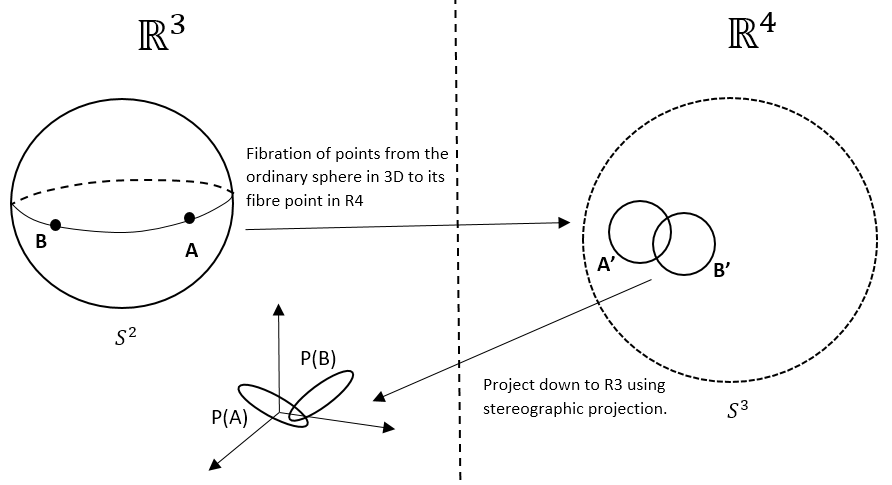
\includegraphics[width=1\linewidth]{hopftheory}}
\caption{Visual process of creating the HF}
\label{fig:speciation}
\end{figure}
\subsection{Hopf Fibration} % Sub-section
%------------------------------------------------
The fourth dimension is a geometric space with four dimensions. Algebraically, the rules of vectors and coordinate geometry is applied to a vector with four components. Which can be used to represent a position in four-dimensional space. But we cannot draw this position, nor can we draw an object.\\

However, we can represent a mapping of an object in four-dimensional space in a similar way a three-dimensional object can be mapped to two-dimensional space. The Hopf fibration (HF) is a representation of the sphere in 4D, in 3D space. The sphere in 4D will be referred to as S$^{3}$. By mapping the 3D surface of the S$^{3}$ in the ordinary 3D space ($\mathbb{R}^{3}$) we will be able to develop a digital 3-dimensional mapping of S$^{3}$ (the HF), which we can use to help us understand the special properties of the S$^{3}$.\\

The HF is a fibration of spheres; the base is the 2-sphere; the fibre is the 1-sphere. With this information about the fibration we can gain detailed visualisations of the 3-sphere. Topology is a field in mathematics where the HF describes the four-dimensional sphere S$^{3}$. Specifically, it is a map from S$^{3}$ to S$^{2}$ where S$^{2}$ is a sphere in $\mathbb{R}^{3}$ . HF is a mapping of the four-dimensional sphere (S$^{3}$). It shows that the S$^{3}$ can be produced by a set of circles that are arranged like points on the 3-dimensional sphere (S$^{2}$).\\
The circles that appear in the HF are known as fibres. The project aims to show the user the symmetry of the HF on a 3D display.  The problem is that this object has been drawn and projected to a 2D display like a monitor. But to experience the best of the beauty of this object, a 3D display would help the user admire and study the properties of the fibration to its fullest in its native dimension. The S$^{2}$ can be described as a shape that is formed of all the points which are of constant distance from a central point. S$^{3}$ is a four-dimensional sphere that is made up of all the points which are constant distance from a centre.\\
This means that the boundary of the S$^{3}$ can collapse into one single point in four dimensions, without collapsing the interior. Imagining the S$^{3}$ can be difficult for us, which is what the HF aims to solve. One way can be a two-dimensional plane of complex dimension, a space with real dimension 4. Where each point in this plane is determined by two coordinates, each coordinate is a complex number. Each axis is a complex line and intersects the S$^{3}$ in a circle. For each complex line that intersects the axis at the origin and S$^{3}$, produces a decomposition of the sphere into circles, known as the Hopf fibration.\\
There are other generalisations of the HF as well. This can be achieved by rotations of the S$^{2}$ in $\mathbb{R}^{3}$ using quaternions which can be identified as H which is also a 4-dimensional space over $\mathbb{R}$.\\
In the classical example, S$^{3}$
is fibered by unit circles in the complex
lines of the standard complex structure on $\mathbb{R}^{4}$. Heinz Hopf showed that this fibration had a map from S$^{3}$ to S$^{2}$. Allowing orthogonal
changes of coordinates, by obtaining other great circle fibrations of S$^{3}$,
each known as a Hopf fibration \cite{Gluck:h}.\\
%------------------------------------------------
\subsection{The Poincar\'e Conjecture} % Sub-section
%------------------------------------------------
The Poincar\'e conjecture is one of the seven problems chosen by the Clay Mathematics Institute as the most important problems of the millennium, and it is the only one that has been solved.\\
This is a closely related topic to the 4-dimensions and the S$^{3}$  surface. The problem was found by Henri Poincar\'e in the early 1900s, which was a question involving topology, the study of shapes and surfaces. During this era of the topology of spheres Poincar\'e claimed there were certain relationships between topology and geometry. It was then found that a loop on any sphere can be contracted to a point. So any closed 3-manifold where such a loop can be contracted to a single point is a S$^{3}$. However, loops on the torus cannot contract to a point.\\
The simple analogy of an apple and a doughnut as given by the Clay Mathematics Institute \cite{clay:pc} helps visualise the problem. By stretching a rubber band around the surface of a sphere (apple), it can be shrunk down to a single point, without breaking the band. If the same were to be done to a doughnut (torus) then we can see that there is no state where the band contracts to a single point. As previously stated; if a loop contracts to a point it is the sphere. Poincar\'e knew that the 2 dimensional sphere is characterised by this property.\\

The basic rules of topology allow us to squash, stretch but the rules of topology do not permit tearing an object, create or close a holes, or joining two points that are not connected, since this will cause things to transform into anything. The sphere has no holes and a torus has exactly one, which is why in topology you cannot form from one of these to another. Poincar\'e had suggested that the object has no holes, is finite, then it can be made into a sphere. This is simple to grasp in 3-dimensions, however, Poincar\'e claims this is true for any number of dimensions.\\

It may be intuitive to think that it must get harder to prove the higher the dimensions, but it is agreed that the proof had gotten harder in the 4-dimensions since it is not as lenient as the higher dimensions. But during the prime time of topology, in the 1960s and 70s, people managed to discover the case of dimension 5 and above though not the 4-dimensional sphere.\\

There have been different approaches to trying to prove the case of 4-dimensions, but many have not succeeded in that it could be said this problem being around for a long period of time has had one of the most failed attempts at proving it. \\

The French mathematician Henri Poincar\'e proposed almost a century ago \cite{johnson:ds} that the world of four dimensions obeys a rule similar to the one that prevails in our world: Things without a hole are just different squishing of the four-dimensional sphere. The technical name for this impossible object is the S$^{3}$. Just as the ordinary sphere is a 2-dimensional surface curving to form an enclosed object in 3-dimensional space, the S$^{3}$ is a three-dimensional surface curving in on itself in four dimensions \cite{johnson:ds}.

One of the first steps taken to solve this was taken by William Thurston, who brought the problem into a more inclusive way that has the Poincar\'e conjecture as a special case \cite{Weisstein:tg}. Even though this was closely related, it was not the proof.\\
The solution was found by Grigoriy Perelman, which was based on Richard Hamilton's theory of Ricci flow. By proving Thurston's geometrization conjuncture, he also proved the Poincar\'e conjuncture which occurs as a special case \cite{clay:pc}.\\

The Ricci flow was invented by Richard Hamilton, which was later used to prove the Poincar\'e Conjuncture. Ricci flow is very closely related to curve shortening flow, which can be thought of by imagining a smooth, closed path and try to deform it such that it becomes a new path. By taking a point on the path and the direction that will move is in the perpendicular of that tangent, which is two directions, in or out. The amount that a point moves actually depends on the severity of the curvature, which can be thought of as the smaller the circle that can be drawn from the path and tangent the tighter the curve and so it will move a lot faster and further. If the point occurs where the circle occurs outside the path, then the direction of the movement will be out. Essentially, the path is expanding and contracting in a flow like behaviour. In the case of a circle; this will contract to a point, at this stage the curvature of the path is arbitrarily big, and forms a singularity and halts.

The same flow in a 3-dimensional surface rather than 2, is called the mean curvature flow. The process is similar to the curve shortening flow but instead we will be expanding and contracting the 2-dimensional surface rather than the 1-dimensional surface. A simple analogy can be a ball that is deflated, instead of a tangent line to describe the surface, there is a tangent plane.\\

Grigori Perelman used something similar called Ricci flow, which looks at the surface of the sphere, not which dimension it is in but defined by a function, such that it can be represented as a matrix for a point. By assigning the metric and changing the metric we can change how we describe the geometry of the surface. For a surface with a lot of curvature the flow will reach a singularity where the cure gets too big. By understanding how this works and how to use it correctly, Perelman was able to solve the Poincar\'e conjucture in the case of the S$^{3}$. \\

The S$^{3}$ is a very complicated object which has taken a century to understand its complicated structure that even dimensions higher than it were solved before it.\\  

%------------------------------------------------
\subsection{Motivation} % Sub-section
%------------------------------------------------
The way we depict the fourth dimension was first discovered around two thousand years ago. The first and simplest extensions of the third dimension (X, Y, Z) was by adding another dimension with the same properties as the others. Known as the Euclidean extension. \\
This was the beginning of higher dimensional geometry. It then leads William Rowan Hamilton in 1834 to discover Quaternions. This is an arithmetic of the fourth dimension, which instantiates the science of Vector analysis. Quaternions are a representation of a four dimensional space.\\
Heinz Hopf discovered the mapping between the 2-sphere and the 3-sphere, known as the Hopf Fibration. The HF is named after Heinz Hopf who studied it in his paper from 1931. He was a German mathematician who worked in the fields of topology and geometry.\\
He discovered the Hopf invariant of maps S$^{3} \,\to\,$ S$^{2}$ and proved that the HF has invariant 1. HF is a map from a higher dimensional sphere to a lower dimensional sphere which is not null-homotopic. Which meant that the S$^{3}$ could be mapped in the form of the Hopf map described as; for any point p on a sphere is mapped to a circle S$^{1}$ in S$^{3}$, however we do not know what this looks like because S$^{3}$ is embedded in $\mathbb{R}^{4}$. But it is possible to map S$^{3}$ to $\mathbb{R}^{3}$.\\
Since this mapping belongs in 3-dimensional space, the motivation is to represent this projection in 3D space. This will mean we must be able to write any point \\
\begin{center}$P = (X1, X2, X3, X4) \in S^{3}$\end{center}
in terms of $p = (x, y, z) \in \mathbb{R}^{3}$. The program intends to help us to understand the structure of the HF and demonstrate the 3-sphere’s symmetry. Unity3D is a cross-platform game engine that can distribute the HF’s stereographic visualisation to many different 3D viewing platforms. \\
The HF visualised in a 3-dimensional space can display a wide variety of different parametrisations. The point p on S$^{2}$, will determine the mapping; these points will be classed as a path on the two-sphere. This can entitle a path to contain points that are not bound by a set. Such a set can have a path around the S$^{2}$ which does mean researching different patterns extracted using equations that take points on the surface of a unit sphere. There are different methods in which you can achieve to draw this shape. But the shape itself has a wide variety of physical applications including magnetic monopoles, rigid body mechanics and quantum information theory. The approach that is popularly taken is the algebra of quaternions but it can also be achieved by complex projective line. \\
Points on the base can be collected in various forms, the usual is a circle sweeping across the horizontal axis which will form a projection of a torus formed from Villarceau circles. The inverse image of a point on the base S$^{2}$ is a Villarceau circle, where multiple points produce the image of linked villarceau circles.\\
 \begin{figure}[H] % Example image
\center{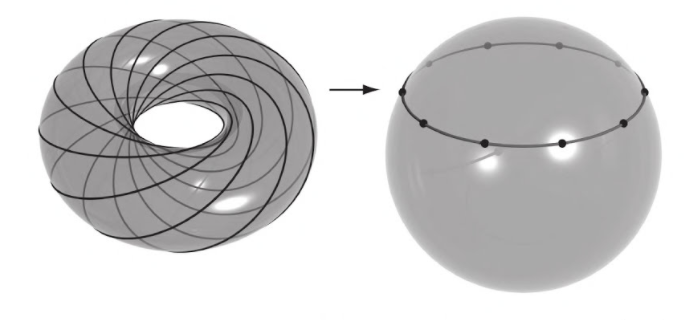
\includegraphics[width=0.5\linewidth]{fibration}}
\caption{Inverse image from the horizontal circle on S$^{2}$ \cite{Walczak:2009dg}}
\label{fig:speciation}
\end{figure}
The motivation is now to let a user decide the base points, which theoretically can produce a set of infinite inverse images, since there is an infinite number of points on the S$^{2}$. This is where Spherical coordinates come of use to define the points on S$^{2}$, this can be fairly cumbersome to do in Cartesian coordinates but with Spherical coordinates it can make programming the base point collection a lot simpler. However, translation from Spherical to Cartesian must also be defined since the fibration of the HF construction defined requires a point in Euclidean 3D space.\\
The formulation of the HF consists primarily on the base points. The program will provide an interaction with the user to define the position of a circle path that can either be vertical or horizontal. The position of the path can be determined by the $\phi$ value given, that represents the angle of elevation in spherical coordinates.\\
The same can be done for vertical circle paths, but this time specifying $\theta$ the polar angle. The program will intend to give the user customisability within the selection of a path, so it can also allow the user to select the length of the path. This will create, for a horizontal circle path, with a length of $\pi$ a half torus. \\
We know that a circle on the base forms a torus after projection, but the number of points on that circle will effect the number of villarceau circle drawn, with a smaller interval between them. The size of that interval should also be left for the user to decide, this can dramatically change to output but visually the shape should still be recognisable, unless the interval is so large only one fibre was drawn. The minimum interval must be trialed so that the user does not create such a large number of points unnecessarily, which can also hinder the performance.\\
Further types of points that can be collected on the base can be in the form of a spiral. The spiral from the northern pole to the southern pole of the S$^{2}$. This means that the user must be able to specify the number of times the spiral will spin around the S$^{2}$. This can be done by specifying values for $k$ and $t$.\\
The spiral on S$^{2}$ can be calculated as
\begin{equation}
(\rho, \theta, \phi) = (1, 2tk\pi, t \pi)
\end{equation}
Since we know the properties of lower dimensional spheres, the principals must be the same. Taking a 3-dimensional sphere and projecting it down to $\mathbb{R}^{2}$ from $\mathbb{R}^{3}$ will result in the projection being a circle. This shows that it is feasible to map a higher dimensional object to a lower dimension. Such that the 4-dimensional sphere can be projected down to $\mathbb{R}^{3}$. Which draws the Hopf map.\\
Bands such as the Mobius band and Hopf band are used to help understand the property and function on fibrations and so better understand the Hopf Fibration. The principles are used to create fascinating orientations of the HF so that the four-dimensional sphere can be pictured in $\mathbb{R}^{3}$.\\

%------------------------------------------------

\subsection{Hopf construction} % Sub-section
%------------------------------------------------
To construct the mapping between S$^{3}$ $\rightarrow$ S$^{2}$ known as the HF, there are three significant stages. The first stage is the Base of the mapping. Secondly, the Fibre formed from the base point. Finally, the projection of the fibration, since we know all fibres can be projected even though it is not formed from a Cartesian product.

\subsubsection{Path on S$^{2}$} % Sub-sub-section
%------------------------------------------------
First we must collect points from  S$^{2}$. These paths have a big impact on the fibration, because this is the primary input that results to produce various features of the HF. If we took all the points on a sphere, then this will fill $\mathbb{R}^{3}$ space. Using different patterns on  S$^{2}$ will result in a different parametrisation of the HF. The different subsets of parametrisations we can find, the more we can find out about the view of HF symmetry.\\ 
The points should be collected using the spherical coordinate system. The coordinates used are $\rho, \theta$ and $\phi$.\\
These coordinates can be translated to Cartesian coordinates as follows:\\
\begin{center}
$
x = \rho \sin \phi \cos \theta \break
y = \rho \sin \phi \sin \theta \break
z = \rho \cos \phi 
$
\end{center}
Rho is the distance from the origin to the point. Theta is the angle in radians between the line from the x-axis and the origin to the point. Phi is the angle between the z-axis and the line from the origin to the point.\\

\begin{figure}[H] % Example image
\center{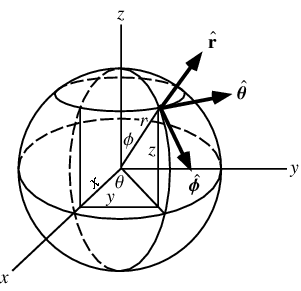
\includegraphics[width=0.4\linewidth]{coords}}
\caption{Spherical coordinate system\cite{Weisstein:sc}}
\label{fig:speciation}
\end{figure}

This coordinate system will make carving out the path on a unit sphere very simple. It is also convertible to Cartesian coordinates. The path of a great circle sweeping on the x-y plane can be constructed by the value of theta iterating\\ 0 $\leq\theta\leq 2\pi$ and $\phi$ and $\rho$ is $\frac{\pi}{2}$ and 1, respectively.\\
The construction of a spiral on S$^{2}$ is defined by the equation stated in the Motivation, which requires the input of $k$ and $t$. The value $k$ which is a constant remains static as it refers to the number of spins the spiral will do before reaching the end of the spiral. The variable $t$ ranges from [0, 1]. The value of $k$ being one will generate a spiral from the top of the S$^{2}$ to the bottom looping around it exactly once. \\
The points collected as a path on S$^{2}$ are base coordinates. An example of a path on S$^{2}$ can be the fibres over a circle of latitude, that forms a torus in S$^{3}$. Projecting multiple circles over different latitudes can produce multiple torus’ in $\mathbb{R}^{3}$ which can fill space if all possible circles of latitude are projected. The torus itself is not constructed by horizontal slices layering the torus, nor is it constructed by arranging vertical circles arranged around in a ring shape (the torus of revolution the result of S$^{1}$ $\times$ S$^{1}$). The torus in the HF made from the circles over a latitude on S$^{2}$, where each individual fibre map to a linking villarceau circles.\\

\begin{figure}[H] % Example image
\center{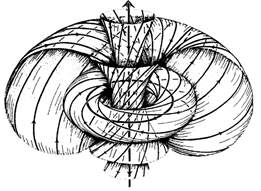
\includegraphics[width=0.5\linewidth]{hopfdrawing}}
\caption{Torus Hopf fibration \cite{Connellan:2014dg}}
\label{fig:speciation}
\end{figure}

Figure 3 is an example of the above description. Each torus represents a circular path where theta is 0 $\leq\theta\leq 2\pi$, sweeping out a circle that lies parallel to the x-y plane.\\

The Hopf fibration is not the only fibration that occurs as a purely fibration of only spheres. In-fact there are four maps including the HF.\\

The typical representation of the HF is where the form follows figure 3, created from the base where each torus in figure 3 is a circle in $\mathbb{R}^{3}$'s unit sphere. These circles can be collected using the spherical coordinate system. However, this is not the only picture that can be formed from the base parameters. In-fact, the unit sphere has infinite possibilities, theoretically.\\  

One of the most fascinating results is where the HF seems to turn its shape inside out. This is a property that can happen in the fourth dimension. Given the correct base values from S$^{2}$ it is possible to construct the HF that shows the 3-sphere turning inside out. Specifically, the base points collected where the circles on S$^{2}$ are vertical, this can show partially the process. The full process is then to rotate those vertical circles along the y axis. At each stage of the rotation there will be a different HF that can be rendered.\\
%------------------------------------------------

\subsubsection{Fibres} % Sub-sub-section
%------------------------------------------------
A fibre or fibration of something means that it can be projected down from the current state. All Cartesian products have a fibre. For example, the Cartesian product of the S$^{1}$ and $\mathbb{R}$ will produce an infinite hollow cylinder. \\
By looking at figure 3, we can simply assume that the HF constructs a torus, which can be easily made by calculating the Cartesian product of S$^{1}$ $\times$ S$^{1}$. However, this is a very different process to the construction of figure 3. The torus shown is primarily constructed using the Hopf link. With enough hopf links we can distinguish the fibration to be a torus.\\

A Mobius band is an example of a non-trivial fibration, the fibration of the Mobius band is one with base S$^{1}$. This means that there is a projection from the mobius band to a circle. This circle can be thought of as cutting through the Mobius in half. The vertical line that is perpendicular to the circle is the fibre. \\

By working backwards, it can be determined that from the circle we can take any point as the base for the mapping then the output will be the vertical line. Therefore, we can take several points as a set from the circle. Which will give us a set of vertical lines that will look like it connects the two circles top and bottom from the Mobius band, hence the fibres. \\


\begin{figure}[H] % Example image
\center{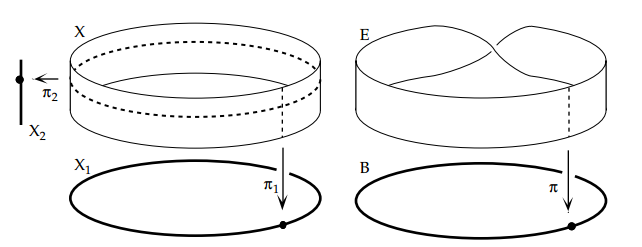
\includegraphics[width=.75\linewidth]{mobiusfibre}}
\caption{fibration of Cartesian and Mobius loop \cite{Ken:q}}
\label{fig:speciation}
\end{figure}

Figure 4 represents one Cartesian band and the Mobius band and their fibre process. The inverse image of the fibre of both the bands will give the S$^{1}$ circle. but the fibre is a line. The fascinating difference between these two examples and the HF and the Hopf band is that everything involved is a sphere.\\

The cylindrical and Mobius bands are fibre bundles but they are topologically different from each other. The twisting nature of the Mobius band means that it is impossible to define a continuous projection to a line since it flips. However, a projection to a circle is feasible. If we imagine that there is a circle running across the centre of the band, where each edge collapses to the centre forming a circle. The inverse image of the point on the circle X1 or B is a vertical line on the band.\\

This is a prime example of the fibre notation and terminology to understand the HF. In terms of the cylindrical band the total space is what the bundle projects onto the base space. The inverse image of each point on the base is what is known as the fibre over the point which is a copy of the fibre space.\\

This may sound confusing but is a reasonably logical approach to understanding what a fibre is. This is the same principal in which the HF fibres the circle, as each inverse image on the base S$^{2}$ gives the point over the fibre which is a circle thus can be projected down to the base space, using stereo-graphic projection.\\

Therefore, we can say that the unit quaternions S$^{3}$ produce fibrations over the S$^{2}$, the unit sphere of $\mathbb{R}^{3}$. Furthermore, a unit vector in the form $q\cdot k \cdot q^{-1}$ will give a quaternion that lies on the S$^{2}$, this is the same as saying three points; $ a, b$ and $c$ associated with an instance of rotation between 0 and 2$\pi$ around the z axis. The fibre produced is a circle, also known as S$^{1}$ in topology.\\

A fibration for the 3-sphere can be explained using a similar process to the one applied for the Mobius band. Instead by using the Hopf band, which is also known as a hopf link, the hopf fibration can be constructed. \\

A property of the HF is that it follows the property of the Hopf band. This band can be visualised by sketching two circular bands that have one link. This is the simplest link with more than one component. The hopf band is an orientable fibration, not like the Mobius band. The hopf and mobius bands are fibrations due to their twisting nature which makes them fibrations but they are not Cartesian products. \\

\begin{center}
\begin{tabular}{| l | l | l |}
\hline
Fibre & Total Space & Base \\ \hline
S$^{0}$ & S$^{1}$ & S$^{1}$ \\ \hline
S$^{1}$ & S$^{3}$ & S$^{2}$ \\ \hline
S$^{3}$ & S$^{7}$ & S$^{4}$ \\ \hline
S$^{7}$ & S$^{15}$ & S$^{8}$ \\ \hline
\end{tabular}
\end{center}

The hopf fibration is not the only fibration of spheres. However, there are only a limited amount of these fibrations that have this property. The creation of these mapping are shown in \cite{Hanson:2006dg}, we will focus on the mapping of S$^{3}$ $\rightarrow$ S$^{2}$. \\
%------------------------------------------------

\subsection{Paremetrisation of Fibres} % Sub-section
%------------------------------------------------
The approaches taken to parameterise the fibres will deal primarily with the S$^{2}$ and S$^{3}$, the unit spheres from $\mathbb{R}^{3}$ and $\mathbb{R}^{4}$. \\
The main goal of this function is to produce a representation of the HF in a 4-dimensional space that can be projected, hence fibre. A fibre is something that has a projection which means that it is capable of displaying to a lower dimension. This property is crucial for the construction of the hopf, because it will allow a 4-dimensional representation to be displayed in 3-dimensions.\\
Each fibre is created from a point from the S$^{2}$, the method of getting these points is shown in the Path on S$^{2}$ section which uses spherical coordinates. The fascinating property is that each fibre is a circle, when projected we can see that two circles can link to form an aesthetically inclined shape. The parameterisation of the fibres can produce a large variety of projections generated from linked circles.
\paragraph{}The two important spheres are the S$^{2}$ and S$^{3}$, the 3 and 4 dimensional unit spheres respectively.
They are defined as follows:\\
\begin{center}
$S^{2} = \left \{ \left ( x, y, z \right ) \in \mathbb{R}^{3} : x^{2} + y^{2} + z^{2} = 1 \right \}$\\
$S^{3} = \left \{ \left ( x, y, z, w \right ) \in \mathbb{R}^{4} : x^{2} + y^{2} + z^{2} + w^{2} = 1 \right \}$\\
\end{center}
The unit sphere is defined as all points 1 unit from the central point. The Base points are also unit points, if not they must be normalised. \\
There are a couple of different approaches that can be taken to achieve the HF mapping. The algebra of quaternions, relates the S$^{3}$ to the S$^{2}$ which is embedded in $\mathbb{R}^{3}$. Another approach is by using C2, which is defined as being in $\mathbb{R}^{4}$, drawing a circle in C2 equates the sphere S$^{3}$ in $\mathbb{R}^{4}$. \\


For the implementation of the S$^{3}$ these values will be used of type Float. Due to the nature of floating point numbers the value will not equal 1 but will be near it.
%------------------------------------------------
\subsection{Interpretation using Quaternions} % Sub-section
%------------------------------------------------
By using S$^{3}$ of unit quaternions to rotate S$^{2}$ we can create the HF. This means we must define a map S$^{3}$ to S$^{2}$. We start by taking a unit quaternion which means $ \left \| q \right \| = 1 $ such that the quaternion is an element of S$^{3}$. Quaternion is equivalent to a rotation matrix representing the HF before projection.\\
Quaternions are an extension of complex numbers, where w, x, y, z are real numbers and i, j and k are imaginary.\\
A fibre over the point $(a, b, c)$ in S$^{2}$ will be determined a rotation $q\theta$ where \\ 0 $\leq\theta\leq 2\pi$ this will draw a circle for each rotation of $\theta$ so long as $(a, b, c)$ is not (1, 0, 0) or (-1, 0, 0).\\
To plot the 3-sphere as a quaternion with the base $(a, b, c)$ and rotation $q\theta$, a possible function is:
\begin{equation}\label{bigboss}
\cfrac{1}{\sqrt{2(1 +\textbf{c})}}\cdot \left( \left( 1 + \textbf{c} \right)\cos( \theta), \textbf{a}\sin(\theta) - \textbf{b}cos(\theta), \textbf{a}\cos(\theta) + \textbf{b}\sin(\theta), (1 + \textbf{c})\cdot \sin(\theta)  \right)
\end{equation}
These fundamental equations form the quaternion algebra
\begin{equation}\label{quaternion}\textbf{i}^2 = \textbf{j}^2 = \textbf{k} = \textbf{ijk} = -1 \end{equation}
The implicit is
\begin{equation}\label{quaternionimp}\textbf{ij} = \textbf{k} = \textbf{-ji}, etc. \end{equation}
This shows that every non-zero quaternion has an inverse which are non-commutative. More can be read at \cite{Kuipers:q}
This function will produce a Quaternion in the form \begin{center}$q = (x, y, z, w) = xi + yj + zk + w$\end{center}
The HF is an example of using Quaternions and the result of it can produce the representation of the HF. The function is the process of finding the fibration of a point S$^{2}$. The Quaternion arithmetic will find the fibration which is something that can be projected, hence the reason why it is called the Hopf Fibration.
%------------------------------------------------
\subsection{Interpretation of 3-Sphere in C2} % Sub-section
%------------------------------------------------
The motivation for this methodology is to think of the sphere S$^{3}$ in C2. We know that the S$^{3}$ is the set of all points at the distance 1 from the origin, in 4-dimensional space. By taking four coordinates from the space the S$^{3}$ equation must satisfy:
\begin{center}$(x_{1}^{2}, y_{1}^{2}, x_{2}^{2}, y_{2}^{2}) = 1$\end{center}

But it can also be thought of as $z_{1} = x_{1} + y_{1}$ and $z_{2} = x_{2} + y_{2}$ being complex numbers. So, we can say that the S$^{3}$ is the pair of complex numbers $(z_{1}, z_{2})$. This means that S$^{3}$ is regarded as the unit sphere in a complex dimension 2, which can be analysed as a circle in a complex plane.\\
For the equation $z_{2} = \textbf{a}\cdot z_{1}$ a defines a complex number such that a line of the form of the equation meets the S$^{3}$ on a circle and so there is a circle for each complex line from the complex number a, the circle will be the fibre.\\

S$^{3}$ in C2 means that the two complex points must satisfy the equation $z_{1}^{2} + z_{2}^{2} = 1$. This means that it can be thought of as the unit sphere S$^{3}$ in complex dimension. From the value 0 on the $z_{2}$ axis a line can be drawn such that it meets with S$^{3}$, which means the value of $z_{1}^{2}$ must be 1. This is of course a complex line that will meet the S$^{3}$ at a circle. Therefore with this methodology it can be concluded that each complex line has its own circle, as the fibration. Similarly, from the Quaternion approach there is a point where $z_{1} = 0$ that cannot feasibly be drawn or projected since it is regarded as being infinite.\\
This proves that the S$^{3}$ is filled with an infinite number of possible fibres that can be drawn since there can be and infinite number of points that can cut the C2 circle resulting in a large variety of aesthetically inclined projections of the HF.\\
This also shows that for each point of S$^{2}$ the points in S$^{3}$ where the image is the point $a$ known as the fibre over $a$ is a circle and so all the points of the line $z_{2} = a\cdot z_{1}$ is simply a constant.
This approach is covered extensively in \cite{Thurston}.
%------------------------------------------------
\newpage
\subsection{Stereographic projection} % Sub-section
%------------------------------------------------
After parameterising the points to a collection of quaternions, the 4-dimensional sphere must be projected to $\mathbb{R}^{3}$. This follows the same principle as projection S$^{2}$ to $\mathbb{R}^{2}$ space.\\
Projection of S$^{2}$ to $\mathbb{R}^{2}$ can be described with a ball in $\mathbb{R}^{3}$ and a light source. By placing the light source above the ball, you will get a shadow on the floor. Similarly, you can project a line from the north of the S$^{2}$ to the projection plane which is n-1 dimension. This can mean that the projection will preserve the circle but the size will be deformed to an extent. Though it is still recognisable as a point in this case.

\begin{figure}[H] % Example image
\center{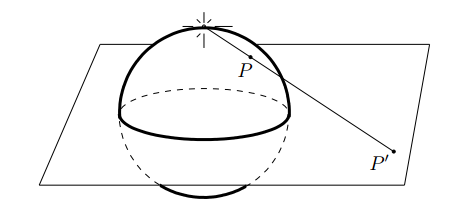
\includegraphics[width=0.5\linewidth]{project}}
\caption{Stereographic projection of S$^{2}$ \cite{Lyons:2003dg} p11}
\label{fig:speciation}
\end{figure}

This is applied to the S$^{3}$ to project it onto a $\mathbb{R}^{3}$ plane, the point will be projected to a point on the plane. A circle of latitude on the S$^{2}$ will be projected as a circle but will not preserve the size, though it is recognisable as a circle. This projection can be done using the equation: \\
\begin{equation}\label{eq:stereo}\large q:(w, x, y, z) \rightarrow \left(\cfrac{y}{1 - w}, \cfrac{x}{1 - w}, \cfrac{z}{1 - w}\right)\end{equation}
The stereographic projection of the point $(0, 0, 1)$ is mapped to a straight line on a plane. The proof for \eqref{eq:stereo} can be found at \cite{Ahlfors:s}
The projection for Unity3D is slightly altered due to the Z axis pointing up, if this stereo-graphic projection was not altered then the construction of the HF will look rotated. 
%------------------------------------------------
\newpage
\subsection{Use of Quaternions in Computer Graphics} % Sub-section
%------------------------------------------------
The discovery of quaternions and their use in computer graphics sparked a revolutionary way of defining camera rotations and animations. Ken Shoemake \cite{Ken:anime} wrote about the use of quaternions in his paper. Many of his publications had used quaternions, especially talking about the fibre bundle S$^{1}$ $\rightarrow$ S$^{3}$ $\rightarrow$ S$^{2}$ such that when a camera tracks an object it does so implicitly operating within the fibre bundle.\\
One of the first representations on computer graphics was a picture made by Ken Shoemake, that was donated to the Hopf topology archive.The picture can be found at \cite{Ken:pic}, which includes an email sent by Ken Shoemake, to the Hopf topology archive describing how it was made.\\

%------------------------------------------------
\subsection{Existing systems} % Sub-section
%------------------------------------------------
There have been many developments to visualise the HF in the past, including Meshview: visualising fourth dimension by Andrew Hanson. This was an interactive visualisation program that was capable of handling 4-dimensional objects. It is able to display 2-dimensional manifolds embedded in 3D or 4D as well as rigid motions from mouse control \cite{Hanson:1999}.\\
The interactive system involved a view and a animation interface to control the a set of polygons and the texture.\\
The aim of this project is to develop on the virtual reality of systems such as this, using new technology to enhance the user's experience of the HF specifically. Though this project will mainly focus on mapping the HF, we will also explore certain methods of visualising colours, and discuss how they relate.
There have been early animations of 4D rotations and manipulations, showing knots in 4D, that is an apparent knot but is not actually a knot can deform into a loop. Hanson's knot$^{4}$ animation \cite{Hanson:vid} describes this clearly by representing the so called knots in 4D with rigid rotations helping to visualise that no knot actually exists. However, the animation shows a family of knotted surfaces that are knotted spheres. The animation shows the object rotating in different angles and colouring parts of the object to help visualise crossing curves on the 3D projections.
%------------------------------------------------
\subsection{Displays} % Sub-section
%------------------------------------------------
Since the HF is a fibration that belongs to $\mathbb{R}^{3}$, stereo-graphic projection will help to ‘get inside’ the fibration to an extent. Stereo-graphic projection will help achieve the HF is displayed in 3D. This also means exploring different applications that may support this and how I must build my project so that it can be integrated to work on different 3D displays.  \\

A 3D TV is a good example of a platform that could host the visualisation of the HF. During the first semester, I have investigated into how to project to a 3D display and compatibility with Unity projects. I have also been involved in an experiment which used a 3D TV to test stereo comfort, by showing me (the subject) different stereo-graphic 3D images. Doing this experiment made me understand what types of problems can occur to cause discomfort to a user and what is very comfortable to look at. \\

To output for a 3D TV, the application must be able to generate two images side by side or top and bottom, for the device to combine. The images must produce a comfortable view of the application, to do this there must be tests completed to find the optimal output. \\

The development in Unity3D mainly aims for, but not only, the Oculus Rift. Virtual reality has become a fast and growing trend in the current era of technology. This project hopes to use this trend in mathematical areas such as topology where virtual shapes can be made to study and admire them and this project aims to achieve this by rendering the HF, a fundamental object in topology.\\


%------------------------------------------------

\subsection{Colours} % Sub-section
%------------------------------------------------
The colour of the HF can vary from fibre to fibre. But the colour can represent different features of the HF. The colour must have a reference to something related to the HF, one example of many can be the latitude of the base points that were collected on the two-sphere.\\
Colour is an interactive feature that the user should be able to change. The meaning of what the colour represents should also be explicit to the user. This feature should allow the user to change the colour reference to their preference.\\
Various colourisation of the HF will increase the interactivity of the program. It will also help users understand the links between the S$^{1}$, S$^{2}$, S$^{3}$ and HF. So far the colours represent either the latitude or the longitude of the base points. \\
The colour of the fibres can be represented from an attribute from the unit Quaternion that corresponds to that specific fibre. This can be done by representing the w value of the quaternion in the HSV colour space \cite{Smith:bre}. \\
This colour space is ideal for the application since most of the values are in unit vectors or quaternions. This means that the hue and saturation values can be one, where the value ranges from 0..1 creating a visual difference but colourful meaning to a fibre.The Quaternion w value can represent the value on the HSV space, because this is a unit quaternion. \\
When a specific point on the HF is clicked the colour of each point on the HF can change to represent the shortest distance from the clicked point from itself, the two points are P and Q. The calculation is to find the smallest angle between the corresponding unit Quaternions.\\
The computation of the shortest distance, between two points P and Q on $S^{3}$, seems relatively straightforward. It is the (smallest) angle between the corresponding unit quaternions:

\begin{equation}\label{eq:colourdistance} \large D(P, Q) = 2(\arccos (P \cdot Q ) )\end{equation} \begin{center}\cite{Hanson:2006ds}\end{center}

The dot product of a clicked component and the Quaternion measuring to, which will be all the other points other than the one clicked is calculated the same way as Euclidean dot product. The result of computing the remaining part of the equation will return a value that lies between 0 and 2$\pi$. \\
In order for this to be used by the HSV colour function, the value is divided by 2$\pi$ bringing the values between 0 and 1.

The HSV model was created by Alvy Ray Smith in 1978. It is a nonlinear transformation of the RGB color space. 
This means that it is not a combination of the primary colours, like the RGB colour space, but is a mathematical transformation.\\
Hue is the is the colour type, red or blue etc. This ranges from 0 to 360 degrees, where the beginning is red. The saturation is the intensity of the colour, this is a percentage of saturation therefore it is from 0-100. The value, or otherwise known as the brightness (HSV is the same as HSB), ranges as a percentage as well so form the value 0 where it is black to 100  which can be white.\\
Since a lot of Unity's other components use the RGB colour space, we must translate our use of HSV that describe the HF properties. This can be achieved by performing the methods described in the founders paper \cite{Smith:bre}.
Thankfully, Unity has a Color class in which a method exists called HSVToRGB \cite{unity:scriptingcolour}. This is a crucial method to use in unity to describe the colour of a fibre, in terms of the properties of the HF. Unity will take the three required values to describe a HSV colour and translate it to a Color object that holds the value in RGB, since the rest of unity's framework uses RGB colour space to define the colour of materials. 
%------------------------------------------------
\subsection{Unity} % Sub-section
%------------------------------------------------
Unity3D supports a cross-platform build engine that provides an intuitive development environment for a 3D or 2D application \cite{unity:manual}. It is used to build applications that follow a game design pattern, which is beneficial for applications that are either focused on animations rather than just logic. With Unity3D a developer does not need to reinvent the wheel. One can simply use the predefined model which Unity3D uses as a template of making a game. \\
Unity3D is known as a Game engine. This means it follows the basic principles of update, rendering and handling threads by encapsulating it the developer can focus purely on their application since the standard setup is completed by Unity3D. 
%------------------------------------------------
\subsubsection{Working in Unity3D} % Sub-section
%------------------------------------------------
The unity environment is suitable for writing scripts and positioning objects that will be used in the application. The environment design can be developed visually by placing objects in the scene. Unity3D provides sufficient tools to edit the objects and even attach scripts to these objects.  \\
The well organised layout and panels can be customised by dragging to a preferred structure. It also provides the opportunity to inspect elements during run-time, to help with debugging the scripts.\\
Unity also provides a pause feature, to control the process of the running application, which also helps with debugging any elements on the scene. It is also possible to inspect the current attribute values of the elements from the scene.\\
Each of the components displayed on the Unity environment are selective panels where each provide different functionalities; the project panel will show all the imported assets and scripts that are used in this project. This is also where you can hold multiple scenes. The hierarchy panel organises the assets and event handlers for the current scene.\\
Scenes manage a set of given assets during its lifetime. The developer can drag items from the project folder to arrange on a specific scene. One asset can be used on multiple scenes. It is also possible to switch between scenes, to emulate moving from the main menu to the visualisation since they are separate scenes.\\
By dragging the asset when the application is paused from runtime from the hierarchy to the project folder, you can create a prefab that can reference multiple instances of that asset. This is a very important functionality that must be used to procedurally generate the fibres of the 3-Sphere.\\
The inspector tab will allow one to inspect or change the object’s attribute values. Since most objects implement the transformation class, this attributes are fully adjustable from the tab. Unity3D allows very detailed adjustments and inclusions. The inspector tab for example, can adjust the convergence and depth properties if the output is to a 3D device via splitting the image left and right.\\
Scripts can give an asset a behaviour. Which is why they can also be called behaviours in Unity. This will give life to an object that it is attached to. A script can be attached to multiple objects that can emulate the same behaviour if that is the goal, simple code reuse.\\
The languages in unity are as follows; C\#, UnityScript (similar to JavaScript) and Boo \cite{unity:scripting}. This project is developed in C\#. \\
Unity is a cross-platform application publisher. It can build a project to Windows, OS X and even to Unity web player which can run on a browser. This is one of the greatest advantages of using Unity, because the application can be developed to a wide variety of platforms it increases the number of potential users and as a developer you do not have to worry about specific platform details too much, since unity encapsulates that.  \\
Unity3D is a very user friendly environment, which helps to provide a seamless experience of development. It provides a lot of support and documentation on how to use Unity3D and its packages appropriately.
The Unity version 5.5 was used to develop the application. This is the latest version at the date of this draft report. This version includes support for development on the Oculus Rift DK2.\\
%------------------------------------------------

%----------------------------------------------------------------------------------------
%	AIMS AND OBJECTIVES
%----------------------------------------------------------------------------------------
%------------------------------------------------
\section{Aims and Objectives}
%------------------------------------------------
The problem of visualising a higher dimensional object is hard to achieve as we live in a space with 3 spacial dimensions. Four special dimensions is the next step. The program should help the user understand more about the four-dimensional sphere and hopefully give them an idea of what it may look like. \\
To develop software that can project the HF and help visualise one of the most important fibrations in topology to solve the problem of visualising and understand better, the four-dimensional sphere in a three-dimensional space.\\
This can be used as an introductory to topology for a mathematician. The HF is one of the fundamental objects in topology. Circles, spheres and tori are among the simplest objects that are studied. A topologist will try to understand the connection between these object, which is what the program will also try to help create. \\
%------------------------------------------------
\subsection{Objectives}
%------------------------------------------------
\begin{enumerate}
\item To undertake research on the four-dimensional sphere so that we can draw a part of it in a three-dimensional space.
\item Build a system that is capable to render the HF to a 3D display. 
\item Implement the program so that it can interact with the user and use the capabilities and functionality of a 3D display. The user must be able to interact with the shape and can look at the fibration in different perspectives. 
\item Design and implement a system that can render the HF efficiently by using any design patterns necessary.
\item Design a feature that will let the user explore many different paths on S$^{2}$ and render what it would look like on S$^{3}$. 
\end{enumerate}
%------------------------------------------------
\subsection{Virtual Reality}
%------------------------------------------------
\subsubsection{The risks}
%------------------------------------------------
Virtual reality is a huge asset to the modern-day world and its development. This new functionality brings a whole new level of products and innovative ideas that can be developed for this platform.\\
However, this does not come without risks. By being aware of the risks that come along with VR, we can develop safe environments that can be used without problems. \\
VR can pose a physical risk to its users. The head tracking functionality may not be very accurate and this can cause motion sickness. This can occur when the user’s head movements are not synchronised well with the HMD such that the response latency is too noticeable.\\
In the past, users have claimed to have had epileptic seizures due to the content synchronisation with the HMD. There are many more potential physical effects; from minor to severe dizziness, seizures. This can potentially cause users a huge shock to users if they were not expecting the reaction. \\
If the virtual reality is done correctly and does not cause these problems, then the application can successfully entertain and represent visual representations of the HF. This can be achieved by following the steps on the risk assessment to ensure the safety of the user and those around.
%------------------------------------------------
\subsubsection{Unity3D}
%------------------------------------------------
Unity supports multiple platforms of Virtual Reality products (\cite{unity:manualvr} includes a list of all supported devices). The support is built into the environment. Unity stated that the VR devices that it offers to build for is a per-platform basis. This means that the application may not work on all platforms depending on the device.\\
A limitation is that only one device can be run at a time. This means that it would not be possible to simultaneously run the application for the Oculus and the 3D TV.\\
Unity has integrated support for Oculus so that it is like a plug and run system, no further packages will need to be installed. Although Unity does recommend to use the Oculus packages for Cameras.

%----------------------------------------------------------------------------------------
%	DESIGN AND IMPLEMENTATION
%----------------------------------------------------------------------------------------
\section{Design and Implementation}
%------------------------------------------------
\subsection{Requirements and Specification} % Sub-section
%------------------------------------------------
The functional and non-functional requirements for the project will determine the path of development and main goals clarified from the project objectives.\\
\subsubsection{Functional} % Sub-sub-section
\begin{enumerate}
\item The application must provide adjustments and input for the Base function and an element of customisability. 
\item The application must be interpretable by a 3D device such as a 3D Television
\item The application must use tubes to represent the fibre 
\item The application must provide a selection of colour preference for the user
\item The application should be able to provide maneuverability for the user’s position so that they can inspect the instance of the HF.
\item The user should be able to click and interact with the HF to discover aspects that should be represented via colour 
\end{enumerate}
\subsubsection{Non-Functional} % Sub-sub-section
\begin{enumerate}
\item The application must be aesthetical and display the visual beauty of the HF
\item The application must run on the Oculus Rift 
\item The application must be able to perform at an acceptable speed 
\item The application must be tested for user comfortability
\item It must project the HF accurately enough so that it can be interpreted
\end{enumerate}
%------------------------------------------------
\subsection{Class Diagram and Design} % Sub-section
%------------------------------------------------
I have produced a class diagram which shows the structure of my design to develop the previously described in chapter 1. The HF is composed of Base points which the class PathsOnS2 will compute over a collection of Point3D objects which have the actual type Spherical. This collection will hold as a path on the two-sphere. The PathAnimator will hold a collection of objects that are of type PathOnS2. A collection will help to distinguish which collection of points belongs to which set of paths. The animator class also holds a collection called HopfLayers; this holds a collection of Fibre objects, which hold a collection four dimensional points which is also referred to as quaternions in the HF construction.  \\
This class diagram will design the HF so that the path on the 2-sphere will be able to update and display an animated visualisation of the HF. The next step is to enhance the features of this design by inhabiting the features of interactivity with the object. To be able to control the viewing aspect (navigation, zoom and other user controls) and to control the HF’s colour scheme, the rotation of the HF (animation) and the paths being collected on S$^{2}$  \\
The Most abstract class that can easily describe the process of the whole system flow is the PathAnimator class. This is attached to the Camera Object in the Hopf Scene. This is so that it will run at the same time as when the Camera is loaded. The Path Animator class will consist of the three major steps described in the Research; Base, Fibration and Projection. This class has the responsibility to manage the connection between the user provided input, saved in the Settings and manipulating the creation of the HF. 
The class is also responsible to listen to any user interaction; such as clicking on the HF after creation. To do this, Unity3D's Update method overridden from MonoBehaviour will help listen to user input at each cycle of the program running.
\begin{figure}[H] % Example image
\center{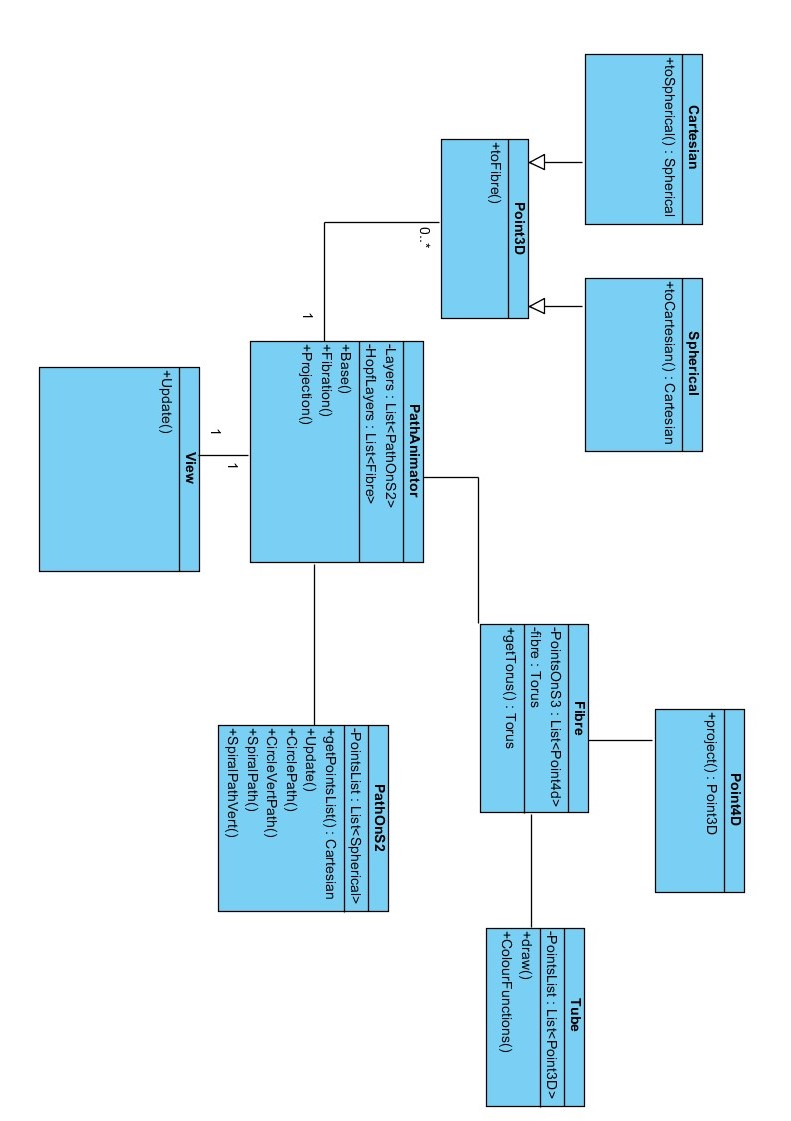
\includegraphics[width=0.9\linewidth]{ClassDiagram}}
\caption{Class diagram}
\label{fig:speciation}
\end{figure}
%------------------------------------------------
\newpage
\subsection{Design patterns and Methodologies} % Sub-section
%------------------------------------------------
A problem or similar problem may have already been solved or abstractly solved. It is a good practice to use design patterns for problems that have similar properties ones that have been solved already.\\
By using design patterns the application can present the structure of the code in a readable and understandable manner. This is very important for not only another developer to understand but for the developer themselves so that they can focus on the core functionalities of the project. \\
Following the prototypical development methodology, the development process was to produce create versions of the application that test and simulate areas of the project functionalities. \\
During the early stages of the development the application can display Base values that are native to S$^{2}$. This was then used to develop the next feature. Therefore, this was a dependent structure where the 3 stages must be tightly coupled. This is to ensure the success of calculating the correct points for the HF. \\

%------------------------------------------------
\subsection{Implementation} % Sub-section
%------------------------------------------------
Developing on Unity allows a developer to have open options about design patterns and implementation styles. The fundamental style for developing in Unity is the behaviour script relationship with the object in a scene. \\
One script can be attached to multiple objects. This can help if two cameras were used each in a different scene, then you only need to write one script for the generic camera which both can be attached to. \\
The implementation style of creating multiple elements of the same object is to have a prefab that is replicated during run-time. It is also possible assign attributes to this object and destroy it if necessary. \\
Generating the points for the HF are all logical procedures, however, to display the HF once the points for the fibre has be calculated, it is ready to be drawn. This was first represented just as a simple line connecting all the points of the fibre. The process took advantage of Unity's LineRenderer component. This is capable of rendering a line given an array of Vector objects. 
%------------------------------------------------
\subsubsection{Abstract pseudo-code} % Sub-sub-section
%------------------------------------------------
\begin{algorithm}[H]
\SetKwInOut{Input}{Input}
\SetKwInOut{Output}{Output}

\underline{function start()}\;
   base()\;
   fibration()\;
   projection()\;

\underline{function base()}\;
\For{$userInput \in inputList$}{
result = new Path()\;
\eIf{$userInput$ == 'circle'}{
\eIf{$userInput.orientation$ == 'vertical'}{
	$result=drawCircle(userInput.phi, userInput.scale, userInput.length)$\;
}{
	$result=drawCircleHorizontal(userInput.phi, userInput.scale, userInput.length)$;
	
}
}{
\eIf{$userInput.orientation$ == 'vertical'}{
	$result = drawSpiral(userInput.spins)$\;
}{
	$result=drawSpiralHorizontal(userInput.spins)$\;
}
}
result.setRotation(userInput.rotation)\;
pathList.Add(result)
}
\caption{The abstract steps in which the HF is constructed, used to implement the program. The Base input of the S$^{2}$ from the user}
\end{algorithm}
This is the abstract way of defining the steps to creating the HF and drawing it. The algorithms follows the three steps discussed in the first chapter. The base function of this algorithm is dependent on the user input, where the user validation is handles at the user entry point, this handles the logic only. The algorithms shows separation between different types of input for a base.
\begin{algorithm}[H]
    \SetKwInOut{Input}{Input}
    \SetKwInOut{Output}{Output}
\underline{function fibration()}\;
\KwResult{perform fibration on each point in the list of paths}
\For{$path \in pathList$}{
	hopfList.Add(path.Fibration())\;
}
    \caption{create a List of lists, where each element in that list is a list of fibration coordinates}
\end{algorithm}

\begin{algorithm}[H]
    \SetKwInOut{Input}{Input}
    \SetKwInOut{Output}{Output}
\underline{function projection()}\;
\KwResult{3D plot-able values}
\For{$list \in hopfList$}{
	\For{$fibre \in list$}{
		Tube tube = new GameObject(Tube)\;
		tube.draw(fibre.project())\;
}
}
    \caption{project each fibre to 3D space and plot onto Unity3D scene}
\end{algorithm}
These are the most abstract layer of implementation, that covers the basic structure of the development and code. The layout follows the mathematical approaches discussed in the first chapter.
%------------------------------------------------
\subsubsection{Fibration pseudo-code} % Sub-sub-section
%------------------------------------------------
\begin{algorithm}[H]
    \SetKwInOut{Input}{Input}
    \SetKwInOut{Output}{Output}

    \underline{function fibrationSet} $(a)$\;
    \Input{point $a$ in $\mathbb{R}^{3}$}
    \Output{List of points in $\mathcal{H} \sim$ $\mathbb{R}^{4}$}
\For{$\omega = scale; \omega < \omega / 2\pi; \omega += scale$}{
	fibrationList.Add(fibrationFormula($a, \omega$))\;
}
    \caption{Quaternion algorithmic approach to defining the Fibration of the pre-image of a point on S$^{2}$}
\end{algorithm}

\begin{algorithm}[H]
    \SetKwInOut{Input}{Input}
    \SetKwInOut{Output}{Output}

    \underline{function fibrationFormula} $(a,b)$\;
    \Input{Point $a$ and the degree of the pole rotation $\omega$}
    \Output{$Point4D$}$
multiplier = 1 / sqrt(2 * (1 + a.z))$\;
$x = multiplier * (1 + a.z) * \cos(\omega)$\;
$y = multiplier * (a.x * \sin(\omega) - a.y * \cos(\omega))$\;
$z = multiplier * (a.x * \cos(\omega) + a.y * \sin(\omega))$\;
$w = multiplier * (1 + a.z) * \sin(\omega)\;$
    \caption{No more further abstractions of the fibration construction. Returns the fibre point Given a point. Equation discussed in chapter 1 \eqref{bigboss}}
\end{algorithm}

%------------------------------------------------
\subsection{Visual Effects} % Sub-section
%------------------------------------------------
\subsubsection{Particle system} % Sub-sub-section
%------------------------------------------------
The particle system does not follow the typical Unity structure for an element. A 3D object is usually represented in the form of meshes. This is the ideal way to represent an object. However, substances that are not solid objects can be cumbersome to portray using meshes and sprites. For effects, such as water or smoke, the particle system is a design that can capture fluidity of the asset.\\
The particles system is used in the project are for a visual effect representing stars around the virtual space. This effect will give the user an immersive feel when using the application. The particles are generated randomly by the particle system.\\
The particles can be small images or simple meshes that are controlled by the particle system that generates a large quantity of particles. The particles in the HF visualisation will represent a star randomly positioned, some of the properties have been altered to fit for use on a 3D device. For example, the clipping distance is slightly further ahead to reduce the chance of eye strain and causing distress to the user. \\
%------------------------------------------------
\subsubsection{Environment} % Sub-sub-section
%------------------------------------------------
The environment can completely change by using a Skybox element. This is a wrapper that goes around the scene creating a long distant scene background effect. Unity also provides customisations to the Skybox, such as adjusting the brightness of the skybox, or changing the rotation.\\
The impression the skybox gives is that it is rendered completely around the scene spherically. However, the skybox only needs six textures to render the scene background. Unity also provides a tessellated sphere to apply textures for more detailed Skyboxes. \\
%------------------------------------------------
\subsubsection{Virtual Menu} % Sub-sub-section
%------------------------------------------------
Since the application is aimed at 3D devices, it is suitable to have an interactive main menu that is not designed typically on Unity2D. The main menu will be split into partial components. Utilising this, the design will be an interactive user menu where the menu is based in 3D where they user is transported to the next sub menu by using packages included in unity; Vector.Lerp, this is a linear interpolation so that the distance is equal between each interval throughout the interpolation, Quaternion.Slerp is a spherical interpolation (Discussed and proved in \cite{Ken:anime}) which is mapped on a segment of a circle which creates a slow-in and slow-out effect. These can be used to transport the user across the menus. But, the user comfortability must not be effected and the speed of the transportation must be adjustable to suit the user.
\begin{figure}[H] % Example image
\center{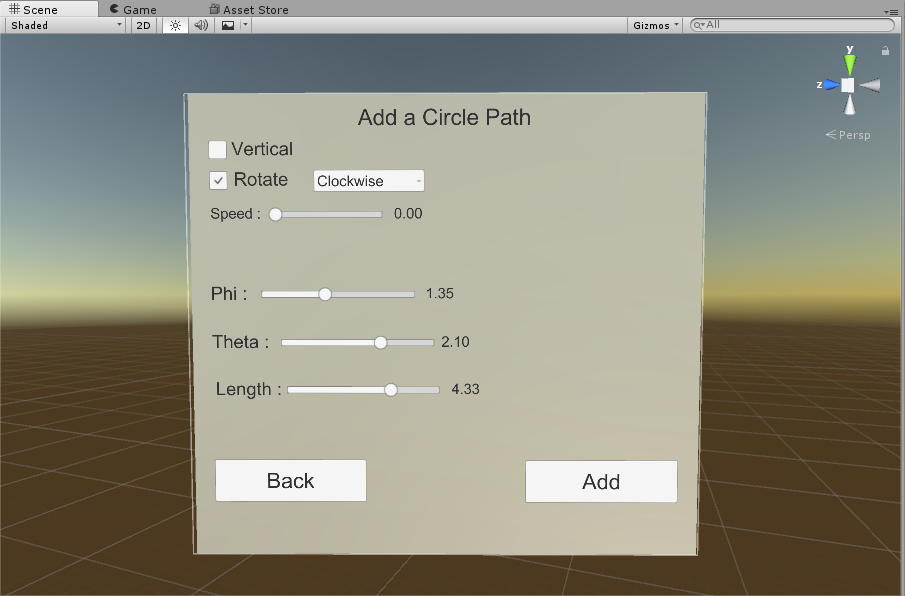
\includegraphics[width=0.75\linewidth]{circlepathmenu}}
\caption{Circle path on S$^{2}$ menu}
\label{fig:speciation}
\end{figure}
The user must be allowed to create a circle path around S$^{2}$, or a spiral path. Both of which can be either vertical or horizontal paths. The Visualise button will open a new world where it will display the current construction of the paths created in S$^{2}$.\\
The circle path menu will let the user edit multiple values relating to the construction by specifying variables in spherical coordinates. The Length attribute shown in figure 6  is the length of how far the theta value if vertical will rotate around to produce a path. The length is from the value 0.1 to 2$\pi$ which is up to all the way around the S$^{2}$, creating a circle. Rotate is a display attribute, if true the object will rotate about the Y axis at the specified speed of rotation. By adding, a S2Input object will be created to store the user's input so that it can generate the path when visualising or calculating the HF. Once a layer of path has been added to the list, it can be visualised to represent what it looks like on the S$^{2}$. 
%------------------------------------------------
\newpage
\subsection{Hopf fibration in Unity} % Sub-section
%------------------------------------------------
The display of The HF will be output to two images; left and right. These images will be rendered as stereoscopic images. This is used to help the 3D device interpret them and combine them so that they can be displayed correctly on the device. Unity allows the developer to tweak the Camera.stereoConvergence, stereoSeperation and stereoEnabled attributes. After Unity’s latest update the scene no longer requires two cameras, but the rendering is calculated by the parameters.
\begin{figure}[H] % Example image
\center{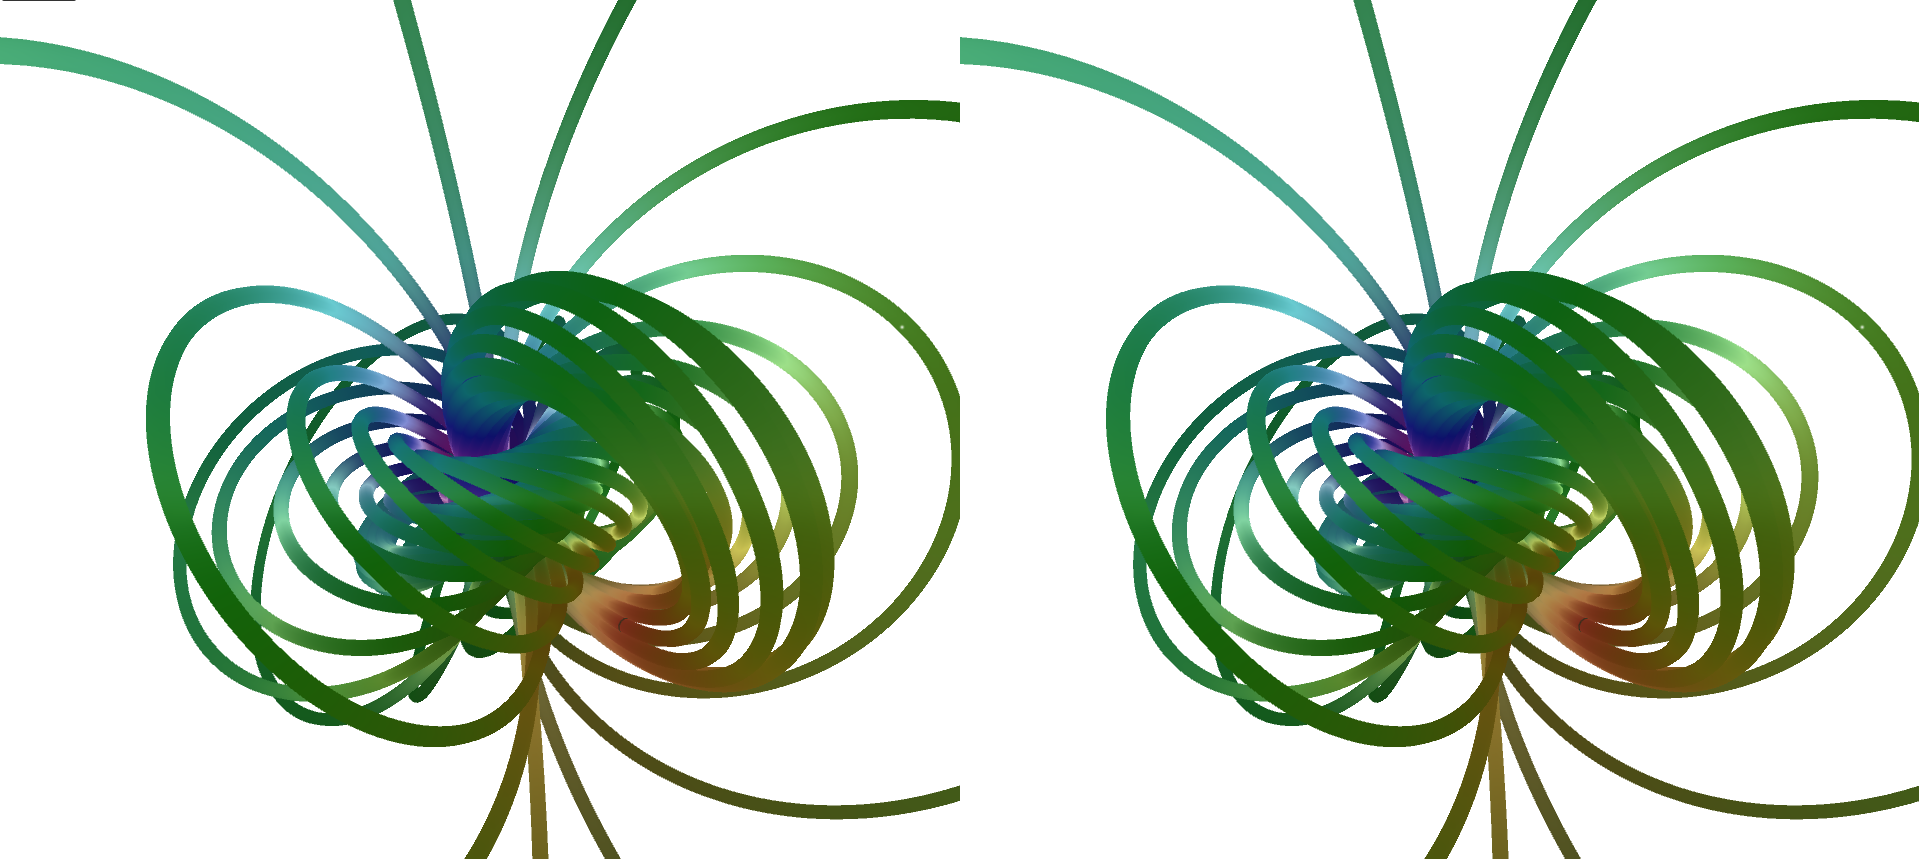
\includegraphics[width=1\linewidth]{stereoview}}
\caption{Stereo enabled view of Hopf fibration}
\label{fig:speciation}
\end{figure}
The HF shown is generated by the set of base points which were a horizontal circle and a spiral around the S$^{2}$ from top to bottom. This construction shows that it is possible to make a HF where each path is a different type. 
The colour here displays the Longitude related to the S$^{2}$ base points. The colour is also set up to change when clicked on the left image, since that is what unity listens to. The right image is plainly view made using the camera stereo parameters.
%------------------------------------------------
\newpage
\subsection{Ray casting for interaction} % Sub-section
%------------------------------------------------
Ray casting is to help the program detect which element the user has clicked on the screen visible to them. This will take the current mouse position on the screen from view coordinates to world coordinates where it casts a ray across a specified length in the world coordinate.\\
This ray will be cast from the origin in the direction set by the mouse position and distance being the maximum distance value. 
To register a click on an object on the scene, Unity3D requires that the object must have a collider mesh to detect collisions. The collider objects will take a similar form to the original component. The collider must also be invisible, which means it does not have to be the same but making it a simpler version will hugely impact the runtime and performance of the application.\\
The RaycastHit object will cast a single ray into the scene. This object will return the information about where the ray hit first
The Raycast in Unity3D also provides an option to include a LayerMask if you wanted to have a blacklist of Collider objects that you do not wish to be hit by a ray.
To make the origin the camera, Unity3D have provided a Ray object that is returned by calling ScreenPointToRay which takes the mouse position as an argument.
For debugging purposes, it can be necessary to include Unity3D's DrawLine once the ray object has been triggered. This can help to visualise where and which direction the ray is casted.
The Ray casting is listened to inside the PathAnimator GameObject. This means that there is a single listener that will only listen for a MouseDown event, which is a GameObject provided by Unity3D. Once this is triggered the PathAnimator will decide what will happen to the point based on the values from the Settings class. The changes will happen to all the Tubes that were saved in the HF generic List when created.
%------------------------------------------------
\newpage
\subsection{Fibre Tubes} % Sub-section
%------------------------------------------------
In the first iteration of creating the HF in Unity3D, I developed a simple program that will take a path that is hard coded into the system and display the output as first the hard-coded path itself that lies on S$^{2}$, then its corresponding HF. \\
The HF drawn in this early iteration of the development used a simple predefined LineRenderer made by Unity3D. This is a simple component that can either take an array of points that is at least of size 2 in 3-dimensions and will draw a line that is the shortest distance between the neighbouring index. Unity3D have enhanced the line renderer to draw complex spirals as well, however this is not relevant for drawing a fibre. \\
 The Line renderer object is a continuous line, which means that a single game object cannot include multiple lines. The simplest solution was to create each fibre as its own game object dynamically depending on the input of the path on S$^{2}$. This means that for the next stage of development, when they are developed into tubes the objects are unique and will be able to have their own Collider Mesh. This will allow the Ray casting object to distinguish which collider it hit and provide detailed information about that specific instance that it hit.\\
The line renderer is a versatile effect that can change the colour, width and material. The colour can be set simply to represent a property of the HF. The width will render the thickness of the line. The line is not a one pixel wise line, but is a set of polygons that will face the camera. \\
The use of LineRenderer was to simply display if the main functions such as; base, fibration and projection were working correctly before committing to render the result in tubes.\\
One of the main requirements was that the fibre was rendered to a tube function, this would mean that it had to be procedurally generated from the points after projection. The projection will output the fibre points in 3-dimensions which may have been rotated, scaled or translated.\\
Since the fibre points could practically be anything, the tube must be able to render a tube at various thickness given a list of points that resemble a circle in Unity3D’s Vector3 object.\\
The tubes, like the line renderer must be able to describe the HF not only by its shape but by the colour. To do this the tube must implement Unity3D’s Mesh and MeshRenderer object and provide them with the necessary inputs so that Unity3D can draw the Mesh.\\
The expected inputs for the MeshRenderer is the geometry from the MeshFilter which will render it from the object’s Transform. The Mesh filter will take a Mesh component, that is usually imported into Unity3D made using 3D designing tools. However, the HF depends on the users input of path which means the tube must be drawn procedurally.
%------------------------------------------------
\subsection{Meshes} % Sub-section
Unity uses meshes to draw and visualise objects.The mesh can either be imported from external packages, or they can be procedurally generated. A mesh is simply a compact structure to draw simple and complex surfaces using triangles.\\
The principal of drawing a mesh follows the rules of triangulation. This is when the surface of some object can be divided into a set of triangles. It was proved in 1925 that every surface can be translated by triangulation, even if it takes an infinite number of triangles \cite{Weisstein:t}. Even though, in computer graphics we can be satisfied with the set of triangles that can be near accurate and also have decent performance.\\
The fibres in the first prototype was drawn using simple LineRenderer. Even this component is actually a mesh that renders billboard lines. These are polygons that are aligned next to each other and always face the camera. This is a very simple component to use in a script since you have to only specify the two points in world space. There are further inputs such as line width and colour that changes the creation of the mesh. The aim is to create a component similar to what the LineRenderer is doing but draws a tube instead of a line given two points.\\
The tube component has a method draw that takes a list of points in the form $(x, y, z)$. to assign values into Unity's mesh object.\\
Unity3D's main graphics component are the Meshes. They are the main graphics primitive for representing objects in world space.\\
The Unity3D's Mesh class allows one to create or modify a mesh using scripts. To create a simple mesh using the Mesh object one could use the user interface in Unity3D, but first the GameObject must have a MeshFilter attached. The mesh filter takes the mesh that is created and assigned to it and passes it to Unity3D's MeshRenderer, which will handle the responsibility of rendering the mesh to the screen.\\
%------------------------------------------------
\subsection{Procedural Meshes} % Sub-section
%------------------------------------------------
%------------------------------------------------
\subsubsection{Tube construction} % Sub-section
%------------------------------------------------
In order to build a mesh from scratch, one must do the following in the correct order \cite{unity:manualmesh};
\begin{enumerate}
\item assign vertices
\item assign triangles
\end{enumerate}
The given list contains points that lie on the same plane, and form a circle; which is the result after the projection of a fibre. This has the vertices for a circle but not a tube. To create a list of vertices for the tube, one must think of each point in the given list is the centre point of a smaller circle.\\
The motivation is somewhat like the TubeGeometry developed in Threejs \cite{threejs:tube}. By taking in the parameters to draw a tube given a set of vectors. Unity has no equivalent though that means we can get our hands dirty in the detailed creation of a procedural fibre.\\
If a circle is drawn for each point then it will form a tube. However, the orientation of the circle matters. This is because a pair of circles (2 points on the fibre list) need to connect to form a triangle between them such that 2 triangles adjacent will form a rectangle.\\
Once the vertices is drawn, the triangles list needs to be created with a size six times larger than the vertices list. This is because each point in the vertices has six entries to form a rectangle where the first point of reference on a click will be the top left index of a quad.\\
A tube is a curved surface therefore the circularity of the tube and the thickness of the tube can only be approximated to represent a tube by using smaller triangles. What we have to admit is that by not making the triangles so small, we can save run-time performance since it will be cumbersome to render such small triangles. \\
Algorithm \ref{six} constructs the array $triangles$ which is six times as large as the array of vertices. The triangles array holds three indexes to represent one triangle, so there are actually three divided by the size of the triangles array. In fact it would be easier Unity had named the array trianglesIndex, because that is what it it. It holds indexes of where to find the vertex of a triangle in the array of vertices. This means the algorithms must keep track of the two arrays and correlate between them. The variables $t$ and $i$ will do just that. The variable $t$ will handle the index value assigned to a triangle at the index of $i$. The reason why it increments by six should be clear since there are six entries per quad. However, the flag is there to make sure to handle array out of bounds, to ensure each tube ring has been circled once without any overlap in the vertices array. Extensive white box testing was carried out to ensure different sizes of tubes are not affected.
%------------------------------------------------
\subsubsection{Tube pseudo-code} % Sub-section
%------------------------------------------------
\begin{algorithm}[H]\label{six}
    \SetKwInOut{Input}{Input}
    \SetKwInOut{Output}{Output}

    \underline{function setTriangles} $()$\;
    \Input{A collection of vertices globally accessible about the tube}
    \Output{List of indexes to the vertices array}
        length = tubeCount * (fibreCount - 1)\;
        triangles = array[length * 6]\;
        flag = 0\;
        \For {int i = 0, t = 0; t < length; i += 6, t++}
        {
            \eIf {flag == tubeCount - 1}
            {
                flag = 0\;
                i -= 6\;
            }
            {
                triangles[i] = t\;
                triangles[i + 1] = tubeCount + t + 1\;
                triangles[i + 2] = tubeCount + t\;
                triangles[i + 3] = t\;
                triangles[i + 4] = t + 1\;
                triangles[i + 5] = tubeCount + t + 1\;
                flag++\;
            }
        }
    \caption{This algorithm will generate an array of indexes that will be used to create mesh triangles. The values stored will be indexes to the vertices array.}
\end{algorithm}
\newpage
The tube is defined by two circles; the larger outline that depicts the fibre as a tube, is known as the $fibreCount$ (effectively holds the size of the input array).
The variable $tubeCount$; is a global variable that holds the number of vertices a circle has to define the width of the tube.

\begin{figure}[H] % Example image
\center{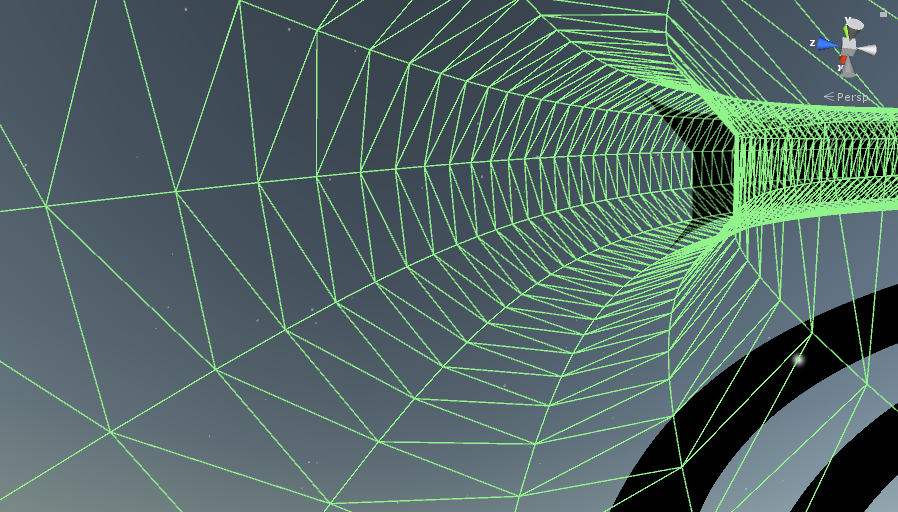
\includegraphics[width=0.75\linewidth]{meshview}}
\caption{Circle theorem for centre and radius given three points on S$^{1}$}
\label{fig:speciation}
\end{figure}

Algorithm 6 shows a simple way of assigning the triangle array with the correct indexes to draw a quad. The difficulty here is to image exactly what is happening during the construction of the tube.\\
If we take two points from the given projected list, $A$ and $B$, where these two points are next to each other in the list. A circle will be generated with the length of $tubeCount$ for each of the points. The point on circle $A$, $a_{1}$ will be the initial point of a quadrant. \\
In Unity, the order of how you assign the three vertices for a triangle will affect the direction the triangle is displayed. Clockwise is vector forward.\\
So from the point $a_{1}$ the next vertex must result in the triangle formed in a clockwise direction. There are multiple intuitive ways of achieving this. Of course this all relies highly on the creating of the circles for each point on the fibre. The points must correlate to form a quad that does not seem to be sheared and must definitely form only a rectangle (of which can also be a square) to connect the two rings.
%------------------------------------------------
\subsubsection{Constructing inner rings} % Sub-sub-section
%------------------------------------------------
One major abstraction that has been assumed so far is the creation of each ring at each point of the fibre. The goal is to generate a circle with a jagged edge that is not too noticeable since it will portray the surface of the tube and also create the ring on such a plane that all the points can be connected to the consequent and preceding rings to form a tube with the same thickness all the way around. This may not seem like a difficult problem, but note that each ring can be drawn in any orientation which can effect the thickness of the tube.\\

By calculating the radius and the centre point, we can find a plane that lies perpendicular to the fibre circle. By using trigonometric functions and circle theorems we can identify the centre and radius as follows;\\
find the vectors $AB, AC, BC$ and its length.\\
\begin{figure}[H] % Example image
\center{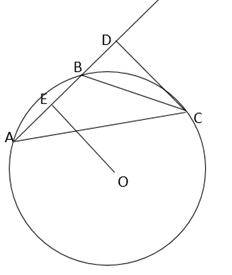
\includegraphics[width=0.3\linewidth]{tubeMaths}}
\caption{Circle theorem for centre and radius given three points on S$^{1}$ which lies on $\mathbb{R}^{3}$}
\label{fig:speciation}
\end{figure}

With three points on the fibre we can find the 3D centre and radius of an arc. Figure 13 and the equations below represent the approach taken. Figure 13 is a 2D drawing of the solution, however the points $A, B$ and $C$ are in 3D space. To find the centre and the radius from 3 points in a 2D space is a lot simpler to compute
\newpage
\begin{equation} \label{eq:someequation}
\cos(BAC) =  \cfrac{AB \cdot AC}{|AB| \times |AC|}
\end{equation}
By finding the angle of BAC we can define another point that then describes the right angle triangle between the two points A and C.
\begin{equation} \label{eq:someequation}
|AD| = |AC| \times \cos(BAC)
\end{equation}
This will hold the length of the hypotenuse, by using trigonometric functions. 
\begin{equation} \label{eq:someequation}
D = A + AD \times \hat{AC}
\end{equation}
By using vector transformations to get the vector to point at the position D giving its point.
We now have the the two lengths $|AD|$ and $|CD|$ and so find the vector $\hat{CD}$.
\begin{equation} \label{eq:someequation}
\hat{CD} = \frac{D - C}{ |CD|}
\end{equation}
this will give the normalised vector $CD$.
\begin{equation} \label{eq:someequation1}
\sin(BAC) = (1 - \cos(BAC))^\frac{1}{2}
\end{equation}
\begin{equation} \label{eq:someequation2}
\sin(BAC) =  \cfrac{AB \times AC}{|AB| \times |AC|}
\end{equation}
The value of $\sin(BAC)$ can be obtained by either of the two methods \eqref{eq:someequation1} and \eqref{eq:someequation2}.
\begin{equation} \label{eq:someequation}
Radius = \frac{|BC|}{2 \times \sin(BAC)}
\end{equation}
We can find the radius using the sine, cosine and ptolemy's theorem \cite{maths:sine}\\
To find the centre point we must define a new variable $E$ that is the midpoint to $AB$.
\begin{equation} \label{eq:someequation}
E.x = \cfrac{|AB|}{2}
\end{equation}
This is simply the midpoint of the $x$ value of $AB$ used to find the centre $x$.
\begin{equation} \label{eq:someequation}
E.y = (R^2 - E.x^2)^\frac{1}{2}
\end{equation}
This will calculate the vector that points to the origin, by using Pythagoras theorem to calculate the y, z values of the origin.
\vfill
\begin{equation} \label{eq:someequation}
Centre = A + E.x \cdot \hat{AC} + E.y \cdot \hat{CD}
\end{equation}
To now draw the ring around the fibre, we must find the cross product of the two vectors $AO$ and $AB$, which will give a perpendicular line to both vectors. \\
By using these vectors as axis, one can draw a circle on the plane made by the cross product result and $AO$ the vector to the radius.
\begin{equation} \label{eq:someequation}
X' = AO \times AB
\end{equation}
\begin{equation} \label{eq:someequation}
Y' = AO
\end{equation}
The vectors $X', Y'$ are perpendicular and have a plane where the ring will be drawn
\begin{equation} \label{eq:circle}
p = centre + (X' \times r \times \cos{\theta}) + (Y' \times r \sin(\theta))
\end{equation}
For equation \eqref{eq:circle} where $r$ is the radius of the ring and $\theta$ ranges from 0 to $2\pi$
%------------------------------------------------

%----------------------------------------------------------------------------------------
%	TESTING
%----------------------------------------------------------------------------------------
\section{Testing}
%------------------------------------------------
\subsection{System performance and requirements testing} % Sub-section
%------------------------------------------------
To generate a large quantity of vertices and render the meshes can take a varying amount of time depending on the different hardware used, and the user input. Unity has developed a system performance program that will check if the hardware, especially the graphics card is capable of rendering for the oculus \cite{douevenrift}. \\
Running the program for the 3D TV, requires a HDMI connection that will supply the display a left and right image. This is achieved by Unity's Stereoscopic rendering mode. Although, this does display to both left and right images, only the left view is interactable.\\
System requirements testing involves the features and testing the user input validity. The user has control over many different functionalities. Stress testing and boundary testing was used to see what values the user can input and how many paths it takes before it becomes unfeasible to draw in reasonable time.\\
A major requirement was to redefine the colours of every fibre vertex relevant to the distance in $\mathbb{R}^{4}$. Therefore, the clicked vertex must be registered and re-render the colours according to their pre-projection state, which is a quaternion.
%------------------------------------------------
\subsection{Results} % Sub-section
%------------------------------------------------
The results consists of images where user inputs various paths on the base. The results also include the output after clicking on a point on the fibration. Clicking on different areas show different properties of the HF.\\
The equation \eqref{eq:colourdistance} calculates the distance between two quaternions. The value is updated as the colour for that vertex's quaternion distance from the clicked quaternion. The distance is the natural distance measure on S$^{3}$, which calculated the geodesic arc connecting them. This value is for unit quaternions and for it to be representable in a HSV colour space, it must be divided by $2\pi$. Images are provided below with a brief description of what the colours mean. However,  
%------------------------------------------------
\subsubsection{Colour distance on click} % Sub-sub-section
%------------------------------------------------
\begin{figure}[H] % Example image
\center{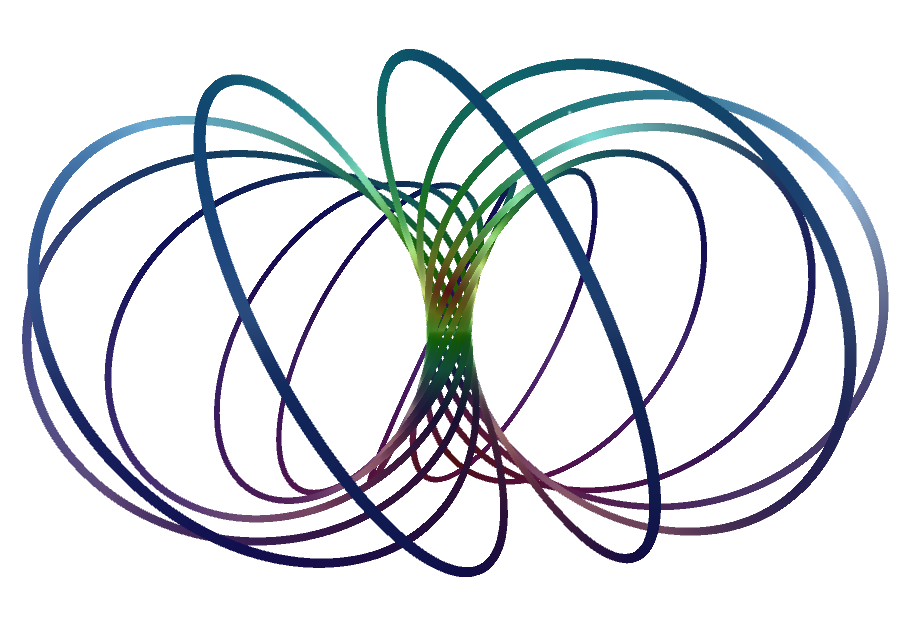
\includegraphics[width=0.5\linewidth]{hopfdist1}}
\caption{colours of fibre represent distance from a central clicked point}
\label{fig:speciation}
\end{figure}

\begin{figure}[H] % Example image
\center{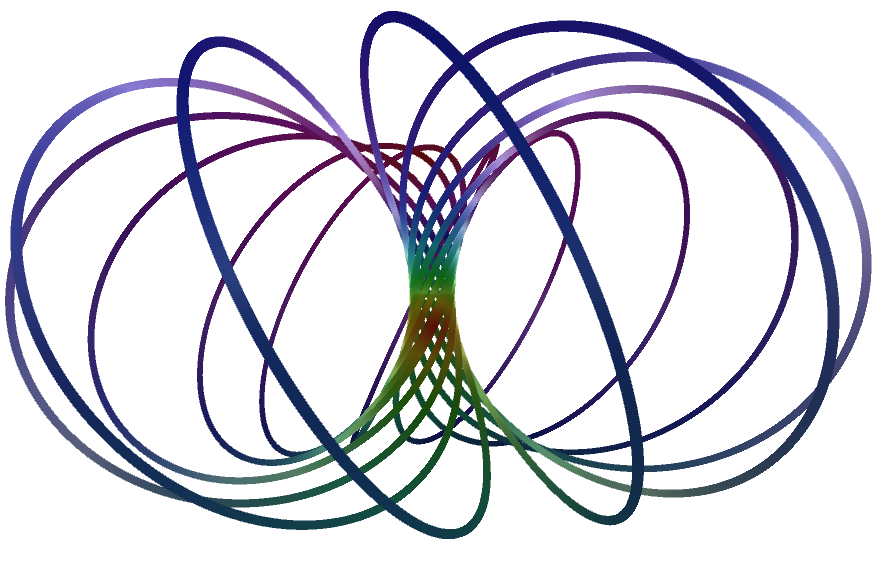
\includegraphics[width=0.5\linewidth]{hopfdist2}}
\caption{colours of fibre represent distance from a central clicked point}
\label{fig:speciation}
\end{figure}
Figures 11 and 12 is the same hopf torus but it has different colours, corresponding to the point at which it was clicked. This shows that the click on a tube works accurately. In accordance to the HSV colour space we can determine that red is the closest and purple the furthest colour. The clicked point for Figure 11 is slightly above the central pillar of the torus. An observation is that the same fibre can be very close and another part of that it is the furthest point. This shows that clicking on different areas of the same fibre can create visual differences. Some of these colours will not make sense if they were calculating the distance between the points in $\mathbb{R}^{3}$. If you consider the Euclidean distance between the red area and the purple area in some cases they seem to have no correlation. If we compare these two colour relations to the inverse image on the S$^{2}$, we can clearly see that the same behaviour has not been orchestrated. Figure 11 and 12 shows that by clicking the centre can cause the northern or southern respectively of the fibre to be the furthest point.  
\begin{figure}[H] % Example image
\center{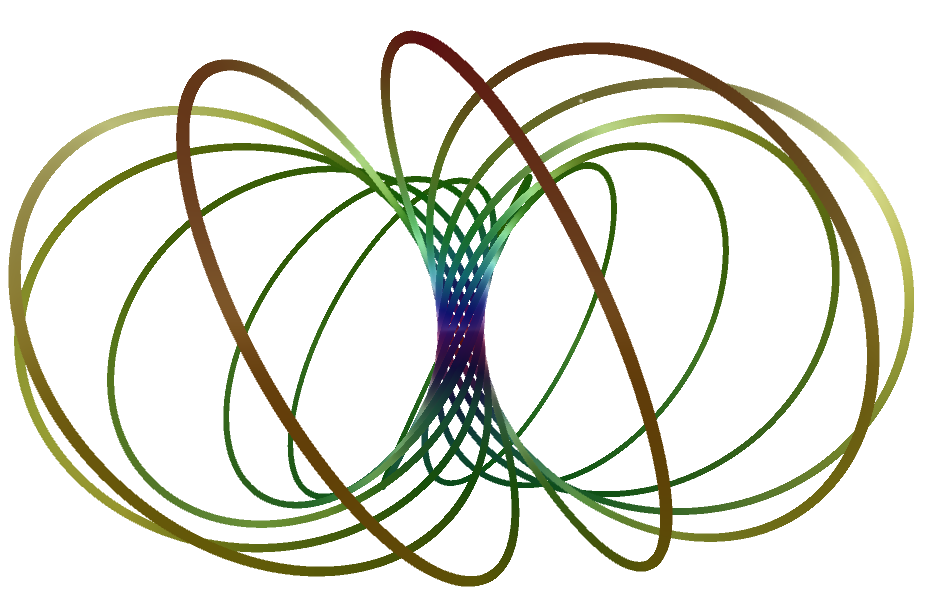
\includegraphics[width=0.5\linewidth]{hopfdist3}}
\caption{colours of fibre represent distance from an outer clicked point}
\label{fig:speciation}
\end{figure}
Clicking near the outer part of the fibre can cause the neighbouring fibres to turn red around the similar area of the tube, however the scale of red is a lot larger than the scale of red from Figures 11 and 12. The scale of red in this image is somewhat similar to the scale of purple in Figure 12. The visible purple in this fibration is from the furthest neighbouring group of fibres, although it only occurs near a group of neighbouring fibres, the rest of the colour of the far set of fibres are of the same colour (green) as the colour of the furthest point from the clicked fibre in Euclidean space.  
%------------------------------------------------
\subsubsection{Latitude and Longitude colours} % Sub-sub-section
%------------------------------------------------
\begin{figure}[H] % Example image
\center{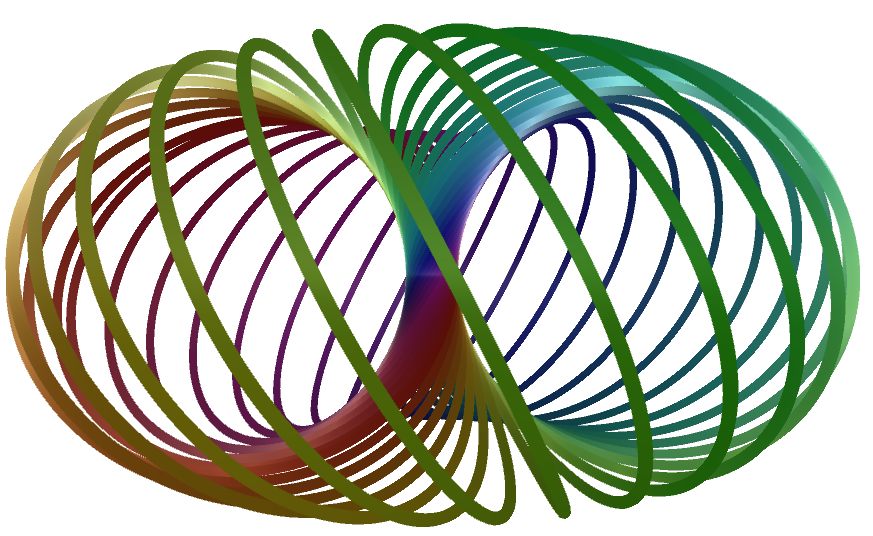
\includegraphics[width=0.5\linewidth]{hopflat}}
\caption{Fibres represent the latitude from the Base points}
\label{fig:speciation}
\end{figure}
The fibres represent the torus with colours across the latitude. This is the correct result since the latitude will vary for each fibre as each point will have a different point of latitude on the base, however the colour of the individual fibre must remain constant throughout that fibre. This figure shows that the statement is true since it colours the fibres in a rainbow like form fully around the torus.
\begin{figure}[H] % Example image
\center{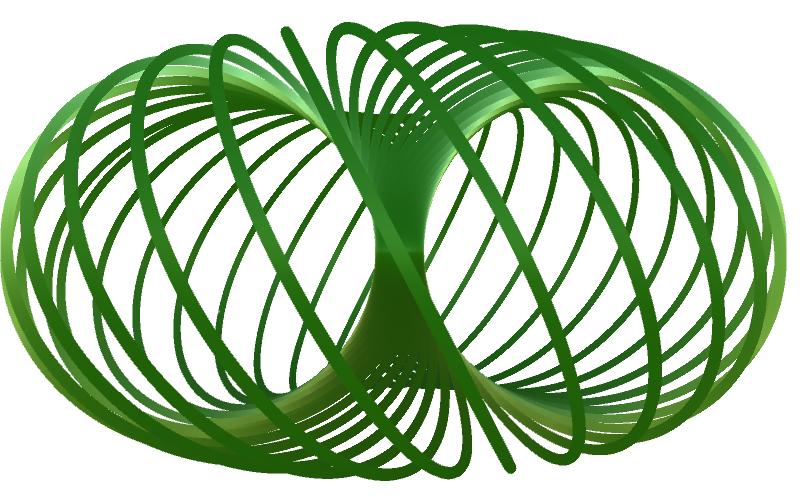
\includegraphics[width=0.5\linewidth]{hopflong}}
\caption{Fibres represent the longitude from the Base points}
\label{fig:speciation}
\end{figure}
The HF is the same base however the colouring function takes the longitude of a point that was taken from the base. This colour should remain constant throughout the fibration since the longitude for the set of points that vertically cut the sphere have the same logitude (are on the same level).
%------------------------------------------------
\subsubsection{Circle path - Horizontal and Vertical} % Sub-sub-section
%------------------------------------------------
\begin{figure}[H] % Example image
\center{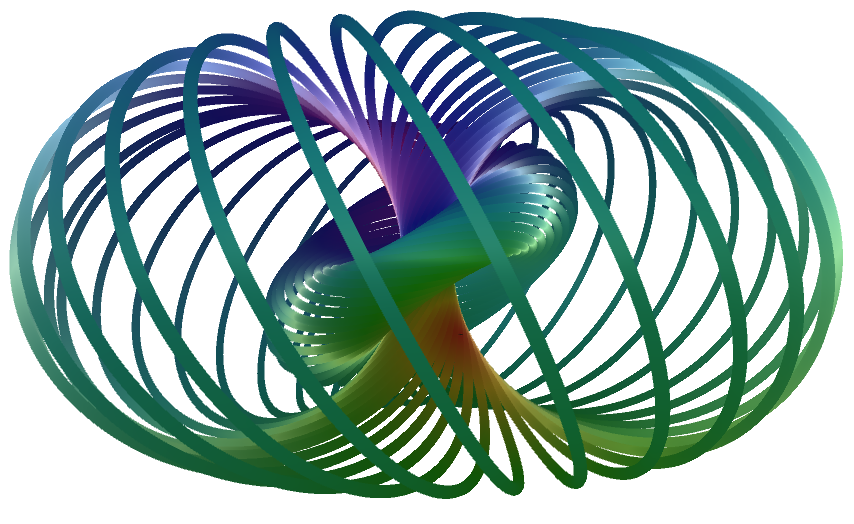
\includegraphics[width=0.5\linewidth]{hopfcirclevh}}
\caption{Horizontal and vertical circles on S$^{2}$ as path}
\label{fig:speciation}
\end{figure}
This shows the HF of two circles; neither of which are intersecting each other, which is also shown in the HF projection. The colouring of this is dependent on the click which was the red area. We can clearly see that there is no visible red area in the second inner torus (made by a vertical circle on the base), this further shows that it has no relevance to Euclidean distance after projection.
%------------------------------------------------
\subsubsection{Spiral path - Horizontal and Vertical} % Sub-sub-section
%------------------------------------------------
The two other options available are vertical and horizontal paths that can be drawn on the base. These are defined by user inputs that require the number of spins, which then will determine the scale at which it should take the points.
\begin{figure}[H] % Example image
\center{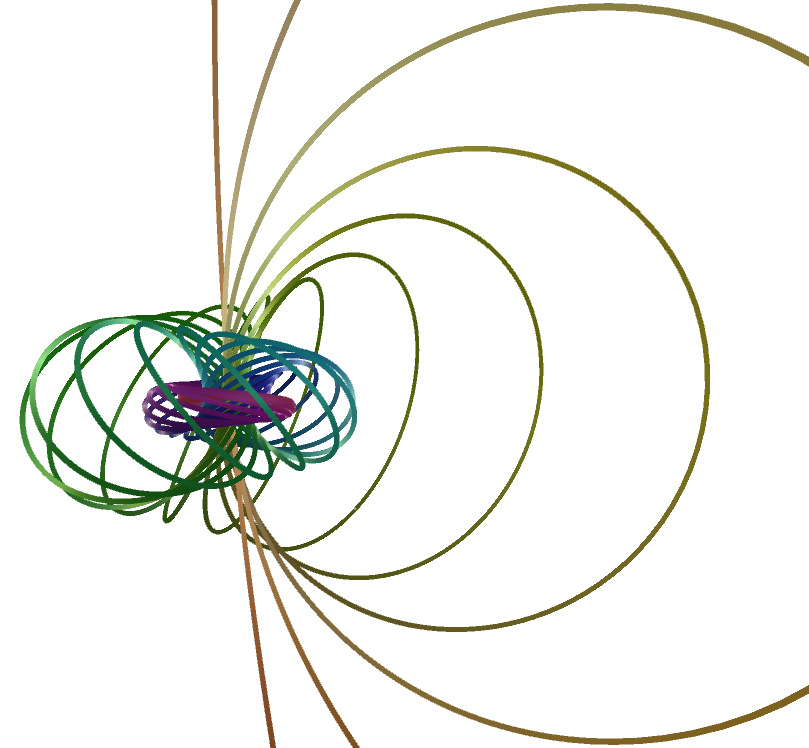
\includegraphics[width=0.5\linewidth]{spiralv}}
\caption{Vertical spiral on S$^{2}$ as path}
\label{fig:speciation}
\end{figure}
As this spiral shows we can see that the circles tend to get smaller as we draw from the top to the bottom, this is best visualised when the creation of the tubes build up. The spiral is simply a fibre taken from every vertical circle from the base as $\phi$ increases at the rate oh [0..1] and the fibre taken from that set has the theta from [0..1] multiplied to $2\pi$, creating a spiral around the sphere a specified amount.
\begin{figure}[H] % Example image
\center{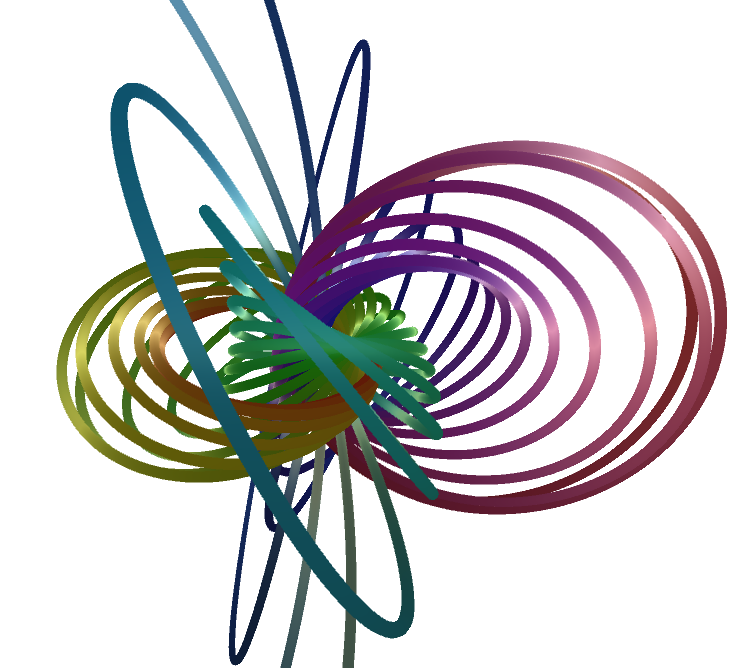
\includegraphics[width=0.5\linewidth]{spiralh}}
\caption{Horizontal spiral on S$^{2}$ as path}
\label{fig:speciation}
\end{figure}
The spiral taking the vertical path is projected in such a way that it shows a torus being able to turn inside-out. This is a common property of many 4-dimensional objects.\\
\paragraph{} Different paremetrisations can produce various results of fibrations to be projected, and  it is possible to project multiple paths at the same time, which will then help the user to visualise from the results given on this platform. With the use of user input and control, a user is able to visualse the base on S$^{2}$ before they encounter the S$^{3}$ so that they can appropriately analyse the results of distances between the equivalent onm S$^{2}$.
%------------------------------------------------

%----------------------------------------------------------------------------------------
%	CONCLUSION
%----------------------------------------------------------------------------------------
\section{Discussion}

%------------------------------------------------
There are many different aspects in which the S$^{3}$ has been used to represent problems and has been involved in some of the most complex problems of the century. The Poincar\'e conjucture has shown that the S$^{3}$ is indeed a complex object. \\
There are further applications that were not discussed in this project, since this is a visualisation of the mapping. By using the mathematical approaches, the HF can be neatly represented on a computer system to display on a 3D device.\\
Being able to develop this for the Oculus meant that the mapping can be displayed in a 3-dimensional platform, giving not only a visual representation of art but science as well. But how can one tell the difference? Through analysis of the results and using proven methodologies, we can be certain the results we have obtained are not just pretty images.
The creation of tubes and meshes have proven to be very challenging, though it was a challenging obstacle, by following software development strategies and the time plan (gantt charts)  I have been able to manage the development efficiently so that all major functionalities were completed and prototypes were improved upon. \\
Working with the HF has encouraged me to use and further apply the use of quaternions in computer graphics for camera rotations especially. With the HF being displayed on the Oculus and 3D TV I have felt developing for these platforms have become extremely versatile, and as a developer you do not have to worry too much about device specific problems and they do not directly effect your system. \\ 
Unity has encapsulates details that can also be altered to some degree; for example, if one was to build a similar system not using a game engine like Unity, they will have to worry about creating camera projections and methods of rendering to a viewport, and even handling the complications of lighting and shading during runtime. Unity takes care of all this and allows the developer to concentrate on what they wish to create. It also provides options to alter these features, such as changing the mode of projection from perspective to orthographic, and the intensity of the lighting.\\
The oculus is a stable device that provides us the capabilities of representing our own 3-dimensional virtual scene and many more projects involving the fourth dimension can utilise this device to enhance the users experience.
%------------------------------------------------
\subsection{Project achievments} % Sub-section
%------------------------------------------------
The project has created a system that can render a projection of the HF, given input from a user. The benefit of deciding to develop this project in Unity has allowed us to display to multiple virtual reality kits that it supports \cite{unity:manualvr} and 3D TVs, through split stereo rendering. The project has also been focusing on creating procedural meshes so that the HF's fibres aren't simple lines but procedural tubes so that the HF can be easily visualised.
TubeRendering function, works as intended to create a circular tube. Although it is possible to purchase such assets from the store that may work similarly, the project has produced its own interpretation since one is not included by standard.\\
The project has also taken into consideration the colouring of the HF, now that it is displayed in 3D, we can distinguish the fibre better than a 2D display. This means we were not restricted to just representing colours of what the base points would have been. For the purpose of visualisation of distances in 4D space, specifically in Quaternions, we have defined a colour function that is capable of colouring the distance of every point from a selected point. This point can be selected by the user.\\
By using development tools and packages only within Unity standard, the project has built a functioning system that meets the requirements set in the previous chapters. \\
The project also uses quaternions for their intended purpose, not just visualisations, instead of Euclidean rotation for camera rotation.\\
The user interface has made use of Unity's user interface tools and designs to create an interactable design on a canvas. The design is created so that it is interactable in a 3D space controlled by camera movements from one 3D menu to another. Since the project is aimed at 3D devices, it only seems fair that the menu and selections also exist in world space rather than having a mundane 2D  space menu that does not react to any head movements from the user wearing the headset.\\
The non-functional requirements are important regardless of the project, as this is what one bases their level of completeness. It is also a measure of how usable the system is as of its intended purpose. Being able to understand the projection of the HF has been achieved since the clicking distance employed is capable of displaying visualisations by implementing distance measures from quaternion space.
%------------------------------------------------
\subsubsection{Personal achievments} % Sub-sub-section
%------------------------------------------------
With no experience from using Unity or C\# prior to the project, this has been a completely new paradigm of programming experience. With a basic background of computer graphics and proficiency in Java it was feasible to develop with the help of a well documented platform. The use use of Unity manual and scripting API have proven to well inform one with no experience in C\# or Unity but has a programming understanding, in a intuitive way of abstracting and encapsulating difficulties. If this project was implemented on just a pure language it would have taken a long time to re-invent the wheel and would not have been feasible to complete the desired outcome in the given time. \\
Unity does not have a TubeRendering asset that comes as standard in the package, there were assets that were at premium price and overly complicated for my intended use. The biggest challenge was problem solving this lack of function and exploring further methods mathematically to find solutions that may help produce a mesh tube with the information about each fibre.
%------------------------------------------------
\subsection{Further development} % Sub-section
%------------------------------------------------
The unity project has incorporated the use of virtual reality to enhance the users interaction experience. Further enhancements to this will be to include a hand controller to control movement, this can help the user move around their heads without having to worry about keyboard inputs, since the inputs on hand held controller are much more ergonomic. Another option could be to make use of the unity's body motion sensor kit that can track body movements to control the direction of movement. Even a CAVE like system, could be a potential enhancement though it may not help understand the HF since output can further stretch or distort giving false output.\\
To include further 4D interactions such as the rotation in 4D controlled by the user. This can be the rotation of the base points rotating after and continually updating the mesh vertices.\\
Another approach could be to let the user decide the path on the base and its rotation, while unity builds this it will render the vertices so that the animation will be smooth and simple to control by a user. Though this may take a longer time and only make short animations.\\
Preset hopf paths that is capable of saving the user's path so that they do not need to re-enter if they wish to see the same fibration.\\
Though the Oculus was used to represent the HF, it can be used to represent other meshes and objects that are natively 4-dimensions, similar to \cite{Hanson:1999} with an enhanced view and similar controls.\\
Currently the visualisation of both the base and the projection cannot be viewed simultaneously. This was thought not to be such good idea since it may cramp the vision of the a HMD user. However, being able to alter base values while visualising a HF can potentially be a promising feature.
Further development will mainly enhance the use of more relevant controls that can potentially help us visualise more aspects of the Hopf fibration, or just to create spectacular fibrations.

%------------------------------------------------
\subsection{Conclusion} % Sub-section
%------------------------------------------------
The Oculus rift and any other VR or 3D device is a revolutionary advancement in technology. These VR devices have sparked a new development era of virtual reality for HMD. Though it comes with stereoscopic risks, there are multiple methods for reducing these discomforts discussed in \cite{discomfort}. The use of Virtual reality really exhibited its advantages in representing the S$^{3}$ by giving the user an extra degree of freedom to move, that feels natural. It was once a nightmare that caused programmers a great ordeal of work to create simple virtual reality software, though with the paired use with Unity3D and the Oculus Rift DK2 goes hand in hand with the 'plug and play' functionality that drastically improved over the previous versions of Unity.\\
With the use of 3D displays such as the Oculus, it meant that a whole new level of design approach can be taken to represent the HF. Effectively having the capability of going inside the fibrations we should be able to click on points and view points that would have been too cumbersome to do on a 2D display. \\
Shapes from the 4D can seem very misleading, especially if being viewed from a 2D display. The collaboration of 3D displays and 4-dimensional representations bring a new dimension, literally, of viewing topological shapes. This approach can help users understand some of the most complex analogies in topology such as deformations and rigid 4D rotations that can reveal behaviours through a visualisation medium in 3D. 

%----------------------------------------------------------------------------------------
%	BIBLIOGRAPHY
%----------------------------------------------------------------------------------------
\newpage
\begin{thebibliography}{99} % Bibliography - this is intentionally simple in this template
\bibitem{Walczak:2009dg}
Walczak, P. et al., 2009.
\newblock {\em Foliations 2012}. Singapore: World Scientific. pp73,83.

\bibitem{Weisstein:sc}
Weisstein, E. W., {\em Spherical Coordinates. MathWorld--A Wolfram Web Resource}. URL: \url{http://mathworld.wolfram.com/SphericalCoordinates.html}

\bibitem{Weisstein:t}Weisstein, E. W., {\em Triangulation}. MathWorld--A Wolfram Web URL:\url{http://mathworld.wolfram.com/Triangulation.html}

\bibitem{Weisstein:tg} Weisstein, E. W. {\em Thurston's Geometrization Conjecture}. MathWorld--A Wolfram Web URL: \url{http://mathworld.wolfram.com/ThurstonsGeometrizationConjecture.html}

\bibitem{Ken:q}
Shoemake, K., 1985. {\em Quaternions}. pp10-12 URL: \url{http://nilesjohnson.net/hopf-articles/Shoemake_quatut.pdf}

\bibitem{Ken:anime}
Shoemake, K., 1985, July. Animating rotation with quaternion curves. {\em ACM SIGGRAPH computer graphics} (Vol. 19, No. 3, pp. 245-254). ACM.

\bibitem{Ken:pic} Shoemake, K., Hopf fibration logo, By Hopf topology archive. URL: \url{http://hopf.math.purdue.edu/new-html/hopflogo.html}

\bibitem{Ahlfors:s}
Ahlfors, L., 1979. {\em Complex Analysis}. 3rd edition. New York:McGraw-Hill. pp18

\bibitem{Gluck:h}Gluck, H. and Warner, F.W., 1983. {\em Great circle fibrations of the three-sphere.} Duke Math. J, 50(1), pp.107-132.

\bibitem{discomfort}Terzić, K. and Hansard, M., 2016. {\em Methods for reducing visual discomfort in stereoscopic 3D: A review}. Signal Processing: Image Communication, 47.

\bibitem{Lyons:2003dg}
Lyons, D. W., 2003.
\newblock An Elementary Introduction to the Hopf Fibration.
\newblock {\em Mathematics Magazine}. pp87-98.

\bibitem{Thurston}
Thurston, W.P. and Levy, S., 1997. {\em Three-dimensional geometry and topology} (Vol. 1). Princeton university press. pp103-106

\bibitem{clay:pc}Clay Mathematics Institute, {\em The Poincaré Conjecture}.
URL: \url{http://www.claymath.org/millennium/Poincare_Conjecture}

\bibitem{johnson:ds}Johnson., G. A. 2003. Mathematician's World of Doughnuts and Spheres. The New York Times.

\bibitem{Kuipers:q}
Kuipers, J.B., 1999. {\em Quaternions and rotation sequences} (Vol. 66). Princeton: Princeton university press.

\bibitem{Hanson:2006ds}
Hanson, A. J., 2006.
\newblock {\em Visualizing Quaternions}.
 San Francisco: Morgan Kaufmann. pp248-249.


\bibitem{Hanson:1999} Hanson, A.J., Ishkov, K.I. and Ma, J.H., 1999. Meshview: Visualizing the fourth dimension. {\em Overview of the MeshView 4D geometry viewer}

\bibitem{Hanson:vid}Hanson, A.J., 1993. 
{\em knotˆ4}. Video animation of knotted
spheres in four dimensions. Siggraph Video Review 93, Scene 1.

\bibitem{Hanson:2006dg}
Hanson, A. J., 2006.
\newblock {\em Visualizing Quaternions}.
 San Francisco: Morgan Kaufmann. pp387-392.

\bibitem{Shokurov:2009dg}
Shokurov, A.V., (originator).
\newblock {\em  Encyclopedia of Mathematics}. URL: \url{http://www.encyclopediaofmath.org/index.php?title=Hopf\_fibration\&oldid=11978}

\bibitem{Connellan:2014dg}
Connellan, L., 2014.
\newblock {\em  Spheres, Hyperspheres and Quaternions}. p18-22.

\bibitem{niles :2014dg}
Johnson, N., 
\newblock {\em Hopf fibration}. 
\newblock URL:
\newblock \url{http://nilesjohnson.net/hopf.html}

\bibitem{maths:sine}Bogomolny, A. 1996. {\em Sine, Cosine, and Ptolemy's Theorem}. Interactive Mathematics Miscellany and Puzzles. URL: \url{http://www.cut-the-knot.org/proofs/sine_cosine.shtml#law}

\bibitem{Smith:bre}Smith, A.R., 1978. {\em Color gamut transform pairs}. ACM Siggraph Computer Graphics, 12(3), pp.12-19.

\bibitem{krap}Krupala, P. nebula skybox. Blender freak. URL:\url{http://www.blenderfreak.com/blog/post/how-to-create-nebula-skybox/}

\bibitem{unity:manual}Technologies, U. 2015. {\em Unity - Manual: Unity Manual}. [online] Docs.unity3d.com. URL: \url{http://docs.unity3d.com/Manual/index.html}

\bibitem{unity:scripting}Technologies, U. 2015. {\em Unity - Scripting API}:. [online] Docs.unity3d.com. URL: \url{http://docs.unity3d.com/ScriptReference/index.html}

\bibitem{unity:scriptingcolour}Technologies, U. 2015. {\em Unity - Scripting API: Colour HSVToRGB} [online] Docs.unity3d.com. URL: \url{https://docs.unity3d.com/ScriptReference/Color.HSVToRGB.html}

\bibitem{unity:manualmesh}Technologies, U. 2015. {\em Unity - Manual: Mesh}. [online] Docs.unity3d.com. URL: \url{https://docs.unity3d.com/Manual/class-Mesh.html}

\bibitem{unity:manualvr}Technologies, U. 2015. {\em Unity - Manual: Virtual Reality}. [online] Docs.unity3d.com. URL: \url{https://docs.unity3d.com/Manual/VirtualReality.html}

\bibitem{unity:manualvr}Technologies, U. 2015. {\em Unity - Manual: Stereoscopic rendering}. [online] Docs.unity3d.com. URL: \url{https://docs.unity3d.com/Manual/StereoscopicRendering.html}

\bibitem{douevenrift} Rift, O. 2015. Oculus VR | Oculus Rift - Compatibility tool. [online] Oculus VR. URL: \url{https://ocul.us/compat-tool}.

\bibitem{douevenriftsupport} Rift, O. 2015. Oculus VR | Oculus Rift - Minimum requirements. [online] Oculus VR. URL: \url{https://support.oculus.com/help/oculus/170128916778795/}.

\bibitem{threejs:tube}Threejs. Tube Geometry. Documentation [online] URL: \url{https://threejs.org/docs/?q=tube#api/geometries/TubeGeometry} [Accessed 10 Jan. 2017].

\end{thebibliography}
%----------------------------------------------------------------------------------------

%----------------------------------------------------------------------------------------
%	APPENDIX
%----------------------------------------------------------------------------------------
\newpage
\section{Appendix}
\subsection{Risk Assessment}
\begin{supertabular}{ p{2.5cm}>{\arraybackslash}p{3.75cm} p{1.75cm} p{1.75cm} p{5cm} }
\hline
Description of Risk & Description of impact  & Likelihood rating & Impact rating & Preventative actions  \\ \midrule
The project requirements are too ambiguous & Can result in producing software that doesn’t align with the specifications & Low & High & Review specifications with supervisor to always check if the project is going on the right tracks.\\ \midrule
Requirements are incomplete & Can lead to confusion when implementing software, cause software to be implemented incorrectly  & Low & Medium & Requirements for my project are straightforward, but it is always good practice to evaluate requirements. \\  \midrule
System outages & Critical systems go down or corrupt data. Can be caused by power cuts, fire, flooding or any other damage corrupting data.& Low & High & Keep backup of program on an external drive in case of any physical or software corruption to original program. \\ \midrule
Components lack of stability & Display or laptop crashing & Medium & High & Make sure the software is compatible with the Oculus rift or 3D display. Check versions and stay updated on display firmware \\ \midrule
Failure to integrate external components & Not being able to use any hardware, hinders the interactivity the program will have. & Low & High & Using software such as Unity3D will ensure compatibility with hardware components such as Oculus Rift and Controllers \\  \midrule
Design lacks flexibility & If the software is designed poorly it can be difficult to make changes & Medium & Medium & Design using UML diagrams to ensure flexibility and feasibility of a task. \\ \midrule
Trailing wires likely to cause trips & Can cause anyone, not only user to trip, that is in the room with trailing wires & High & High & Wires to be covered where possible, appropriately by cable management equipment. Where trailing wires are unavoidable, they must be identified to any personnel entering the room. \\  \midrule
Occlusion of vision when using Oculus Rift & The user will not be able to see any obstructions and obstacles in their surroundings. Can cause injury. & Medium & High & Assess the room and space before using the Oculus Rift, making sure the environment is suitable. The Oculus Rift is tethered to a computer therefore it must be used seated. \\ \midrule
Prolonged use may cause nausea and dizziness & Use of the Oculus rift can potentially cause the user to get dizzy, blurred vision or any other adverse effects caused by the Oculus Rift or other 3D displays & High  & High & All of the users must be advised of the potential adverse effects that occur, before use. If any of the problems do occur; eye strain, dizziness, blurred vision or nausea then stop use of system immediately. User is advised to use the 3D device for no longer than 15 minutes without a break. \\ \midrule
\end{supertabular}
%------------------------------------------------


\end{flushleft}
\end{document}